\documentclass{article}

\PassOptionsToPackage{numbers,sort&compress}{natbib}
\usepackage[preprint]{neurips_2021}
\usepackage[utf8]{inputenc}
\usepackage[T1]{fontenc}
\usepackage{hyperref}
\usepackage{url}
\usepackage{booktabs}
\usepackage{microtype}
\usepackage{xcolor}
\usepackage{graphicx}
\usepackage{subcaption}
\usepackage{multirow}
\usepackage{array}
\usepackage{adjustbox}
\usepackage{enumitem}
\usepackage{algorithm}
\usepackage{algpseudocode}
\usepackage{amsmath}
\usepackage{amssymb}
\usepackage{amsfonts}
\usepackage{amsthm}
\usepackage{mathtools}
\usepackage{bm}

\title{CDA: Post-hoc Domain Generalization by Seeking Distributional Canalization}

\author{
Jayden Jeong\\
Math Science Technology Center\\
Paul Laurence Dunbar High School\\
Lexington, Kentucky\\
\And
Vijayan K. Asari\\
Vision Lab\\
University of Dayton\\
Dayton, Ohio
}

\newtheorem{theorem}{Theorem}[section]
\newtheorem{proposition}[theorem]{Proposition}
\newtheorem{lemma}[theorem]{Lemma}
\newtheorem{corollary}[theorem]{Corollary}
\newtheorem{assumption}[theorem]{Assumption}
\theoremstyle{definition}
\newtheorem{definition}[theorem]{Definition}
\newtheorem{remark}[theorem]{Remark}

\newcommand{\RR}{\mathbb{R}}
\newcommand{\EE}{\mathbb{E}}
\newcommand{\cA}{\mathcal{A}}
\newcommand{\cB}{\mathcal{B}}
\newcommand{\cC}{\mathcal{C}}
\newcommand{\cD}{\mathcal{D}}
\newcommand{\cE}{\mathcal{E}}
\newcommand{\cF}{\mathcal{F}}
\newcommand{\cG}{\mathcal{G}}
\newcommand{\cH}{\mathcal{H}}
\newcommand{\cN}{\mathcal{N}}
\newcommand{\cS}{\mathcal{S}}
\newcommand{\cT}{\mathcal{T}}
\newcommand{\cV}{\mathcal{V}}
\newcommand{\cW}{\mathcal{W}}
\newcommand{\argmin}{\operatorname*{arg\,min}}
\newcommand{\argmax}{\operatorname*{arg\,max}}
\newcommand{\Var}{\operatorname{Var}}
\newcommand{\KL}{\operatorname{KL}}
\newcommand{\diag}{\operatorname{diag}}
\newcommand{\simplex}{\Delta}
\newcommand{\one}{\mathbf{1}}
\newcommand{\eps}{\varepsilon}
\newcommand{\cda}{\textup{\textsc{CDA}}}
\newcommand{\vsc}{\textup{\textsc{VSC}}}
\newcommand{\piv}{\textup{\textsc{CDA-Piv}}}
\newcommand{\bd}{\textup{\textsc{CDA-BD}}}
\newcommand{\erm}{\textup{\textsc{ERM}}}
\newcommand{\swad}{\textup{\textsc{SWAD}}}
\newcommand{\diwa}{\textup{\textsc{DiWA}}}
\newcommand{\eoa}{\textup{\textsc{EoA}}}
\newcommand{\ood}{\textup{\textsc{OOD}}}
\newcommand{\norm}[1]{\left\lVert #1 \right\rVert}
\newcommand{\abs}[1]{\left\lvert #1 \right\rvert}
\newcommand{\inner}[2]{\left\langle #1, #2 \right\rangle}
\newcommand{\paren}[1]{\left( #1 \right)}
\newcommand{\braces}[1]{\left\{ #1 \right\}}
\newcommand{\ub}{u_E}
\newcommand{\thetaw}{\bar{\theta}(w)}

\begin{document}

\maketitle

\begin{abstract}
Post-hoc domain generalization has produced strong empirical methods, but its explanations remain fragmented: some methods emphasize flatness, others emphasize diversity, and others rely on validation selection. We propose \emph{distributional canalization} as a common source-side principle for this regime. A model is canalized when its source risk is stable under small redistributions of source-domain mass. Under a source-supported hidden-shift assumption, we prove that target risk is upper bounded by mean source risk plus a source-mixture sensitivity term. This recovers flatness as a sufficient condition for safe averaging, explains when diversity helps through cancellation of centered domain-response vectors, and motivates non-contiguous checkpoint families when they preserve the source-support disagreement structure needed to control the certificate. We then instantiate this principle in a checkpoint-bank method with three components: a version-space compression selector that retains a non-contiguous family preserving full-bank threshold disagreement, a pivotality-shift weighting rule derived as a first-order canalization proxy, and a Blackwell-inspired dual weighting rule that moves the source-loss vector toward the per-domain best-loss target set with entropy regularization. On PACS replay experiments, the fixed version-space selector retains non-singleton families on all four target splits, and the two CDA-derived weight rules reach mean full / in / out accuracies of \(88.43/88.24/89.16\) and \(88.42/88.22/89.20\), respectively. On the art-focused family sweeps, these post-hoc weighting rules yield modest but real gains over the corresponding plain uniform family soups. The result is not an unconditional guarantee of target superiority; it is a theory-grounded, source-only criterion for choosing which post-hoc soups are plausible under hidden source-mixture shift.
\end{abstract}

\section{Introduction}

Modern domain generalization methods are often evaluated by their ability to improve an already-strong empirical risk minimization pipeline without using target-domain data. Post-hoc methods are especially attractive in that setting. A single training run produces a trajectory of checkpoints, and the final deployed model is selected or averaged only after training. This avoids modifying the base training algorithm, but it creates a new scientific question: what source-only quantity should decide which post-hoc model is deployed?

That question is easy to understate. Training-time domain generalization methods can alter the representation, the loss, or the data pipeline, so their inductive bias is distributed across the whole optimization process. Post-hoc domain generalization does not have that freedom. It receives a completed checkpoint bank and must choose one deployable model using only source-domain evidence. This makes post-hoc DG unusually interpretable, because the selection rule is concentrated in one place, but it also makes the theory unforgiving: if the rule is wrong, there is no later training stage that can repair it.

The literature gives several partial answers. Flatness-based post-hoc methods argue that broad valleys are safer under shift, and checkpoint averaging methods exploit the empirical fact that weight-space averaging can land inside a robust region when the averaged checkpoints are locally compatible \citep{izmailov2018swa,garipov2018mode,frankle2020linear,cha2021swad,wortsman2022soups}. Diversity-based methods argue that averaging should combine models whose errors are not redundant, so that one checkpoint can compensate for another under distribution shift \citep{rame2022diwa,arpit2022eoa}. Model-selection work warns that without target labels, source validation can be a weak proxy unless the selection rule captures the right invariances and failure modes \citep{gulrajani2021domainbed}. These perspectives are useful, but they are usually presented as separate intuitions.

This paper argues that a more fundamental object is \emph{source-mixture sensitivity}. In the source-only regime, the target domain is unavailable, but source data contain multiple environments and subpopulations. A natural local hidden-shift model says that the target behaves like a nearby redistribution of source-domain mass, up to an approximation error. Under that model, the deployable predictor should not only have low average source loss; it should be stable when the weights of the source domains are perturbed. We call this property \emph{distributional canalization}. The phrase is meant literally: a canalized model channels nearby source-mixture perturbations into small changes in risk.

The motivation is not merely aesthetic. In many DG settings, the source domains are already broad aggregates, such as PACS domains or DomainBed environment splits. A validation loss that averages them uniformly can hide a real structural weakness: the model may be excellent on the dominant source modes and brittle on the minority modes that are most relevant to the unseen target. Conversely, a selector that optimizes only the worst source domain can be too pessimistic when the final deployable soup is allowed to average complementary checkpoints. The source-only criterion therefore needs to be richer than either pure averaging or pure worst-domain selection.

This view unifies several empirical motifs. Flatness helps because if the soup remains in a region where each source-domain loss is locally stable, the mergeability remainder is small. Diversity helps only in a sharper sense: centered domain-response vectors must cancel under the chosen weights. Arbitrary diversity in parameter space is not enough. Non-contiguous averaging can be valid because the theorem does not require checkpoints to be adjacent in training time; it requires the retained family to preserve the source-side disagreement and domain-response geometry relevant to the hidden-shift certificate.

That last point matters in practice. Much of the checkpoint-averaging literature inherits an implicit contiguity bias from stochastic weight averaging and related methods: late checkpoints are averaged because they are nearby in parameter space and therefore expected to be averageable. But a completed checkpoint bank contains other structures besides temporal adjacency. If two checkpoints are far apart in training time yet share the same source-support disagreement geometry and remain mergeable under averaging, a source-only certificate has no reason to discard them purely because they are non-contiguous. One aim of this paper is to make that statement mathematically explicit.

The practical method studied here uses a dense checkpoint bank from one training run and builds one deployable weight soup. It has three parts. First, the \emph{version-space compression} selector greedily retains a non-contiguous subset that preserves the full bank's threshold-disagreement mask over source-support true-class probabilities. Second, \piv{} assigns larger weights to checkpoints that are pivotal under leave-one-out removal while penalizing source-mixture sensitivity. Third, \bd{} optimizes the source-domain loss vector toward the coordinatewise best source-domain loss target, with entropy regularization to avoid unnecessarily sharp weights. These are not independent tricks; each is derived as a practical relaxation of the canalization certificate.

The manuscript is careful about the scope of its claims. We do not claim an unconditional superiority theorem over other DG methods, nor do we claim that local source-mixture shift is the only relevant model of target variation. The claim is narrower and more defensible: if one works in the source-only post-hoc regime and accepts a local source-supported hidden-shift model, then distributional canalization is a coherent criterion, and the resulting selector-weighting pipeline gives a principled way to search a checkpoint bank.

\paragraph{Contributions.}
The paper makes the following contributions.
\begin{enumerate}[leftmargin=1.4em]
    \item We formalize distributional canalization as a source-only target-risk certificate under local hidden source-mixture shift.
    \item We derive exact variance and pairwise-interaction decompositions showing when diversity reduces hidden-shift sensitivity, and we prove a low-curvature mergeability result explaining why flatness-based averaging can work.
    \item We introduce a version-space compression selector for checkpoint banks and give a compression-style bound showing how disagreement preservation trades family size against certificate error.
    \item We derive \piv{} and \bd{} as two weighting rules from the same canalization premise: one as a first-order pivotality-plus-sensitivity proxy, the other as a Blackwell-inspired target-set relaxation.
    \item We provide PACS replay evidence showing that the resulting non-contiguous families and source-only weights remain competitive across all four completed PACS target splits, and that on the art-focused family sweeps they modestly improve over the corresponding uniform family soups while retaining a clear limitation profile.
\end{enumerate}

\paragraph{Roadmap.}
Sections~\ref{sec:theory}--\ref{sec:weights} develop the theory and the selector-weighting construction. Section~\ref{sec:method_overview} consolidates the practical pipeline. Section~\ref{sec:experiments} presents the PACS replay evidence and explains why the paper reports the VSC selector rather than the strongest art-only selector. The appendix collects fuller proofs, diagnostics, and implementation details.

\begin{figure}[t]
    \centering
    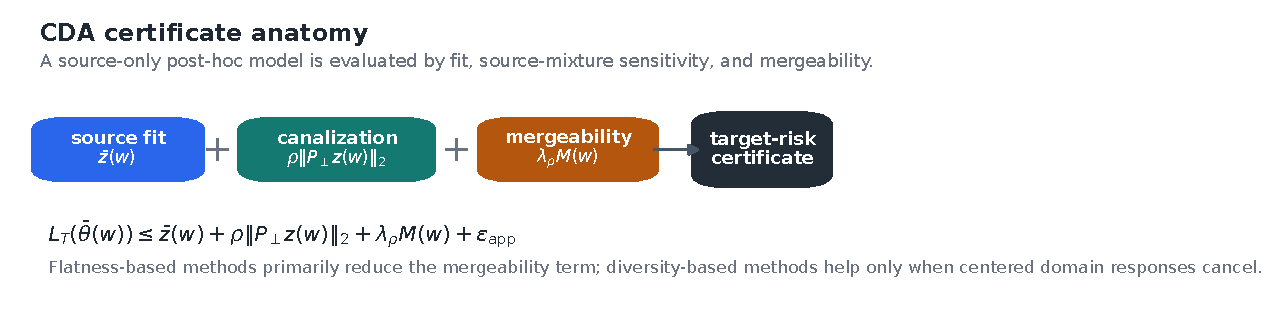
\includegraphics[width=\linewidth]{figures/certificate_anatomy.pdf}
    \caption{\textbf{CDA certificate anatomy.} The target-risk certificate decomposes into source fit, source-mixture sensitivity, and a mergeability remainder. Flatness-based methods primarily control the mergeability term. Diversity-based methods help when centered domain responses cancel under the chosen weights.}
    \label{fig:certificate}
\end{figure}

\section{Related Work}

\paragraph{Domain generalization and model selection.}
DomainBed showed that domain generalization algorithms must be compared under careful model-selection protocols, because many apparent gains disappear under controlled evaluation \citep{gulrajani2021domainbed}. PACS remains a common benchmark for visual domain shift across art painting, cartoon, photo, and sketch domains \citep{li2017deeper}. Classical domain adaptation theory also makes clear that source-only learning cannot control arbitrary target shifts without assumptions linking source and target distributions \citep{ben2010theory}. Our analysis is explicit about this point: the target-risk certificate assumes a local source-supported hidden shift.

The distinction between training-time DG and post-hoc DG is especially important here. Training-time methods can improve invariance by changing data augmentation, optimization, or the representation itself. Post-hoc methods accept the representation and the bank as fixed. This makes them appealing in high-compute settings, where retraining is expensive, but it also means their scientific content is concentrated in a small number of source-only decisions: which checkpoints to keep, how to weight them, and what source-side evidence is trusted. A real theory for post-hoc DG therefore has to address these choices directly rather than inherit them from the training procedure.

\paragraph{Flatness-based post-hoc averaging.}
Stochastic weight averaging connects weight averaging to broad optima and improved generalization \citep{izmailov2018swa}. Mode connectivity and linear mode connectivity show that independently trained or trajectory-adjacent models can sometimes be joined by low-loss paths \citep{garipov2018mode,frankle2020linear}. Model soups show that averaging fine-tuned models can improve accuracy without increasing inference cost \citep{wortsman2022soups}. In domain generalization, \swad{} uses dense weight averaging to seek flatter minima and reports strong DomainBed results \citep{cha2021swad}. CDA keeps the flatness insight but reframes it: flatness is useful because it controls the mergeability remainder in a source-mixture certificate.

This reframing matters because flatness, by itself, says little about \emph{which} source directions matter. Two soups can look equally flat under pooled loss while behaving very differently under domain-weight perturbations. A post-hoc DG criterion should therefore be able to say when flatness is relevant and when it is insufficient. Our low-curvature proposition and pooled-flatness separation result are aimed precisely at that distinction.

\paragraph{Diversity-based post-hoc averaging.}
\diwa{} emphasizes functional diversity and locality for out-of-distribution weight averaging \citep{rame2022diwa}. \eoa{} studies ensembles of averaged models and improves post-hoc model selection in domain generalization \citep{arpit2022eoa}. CDA provides a complementary mathematical lens: diversity matters when it reduces the norm of the weighted centered source-domain loss vector. The relevant object is not diversity alone, but cancellation of domain-response directions that correspond to plausible source-mixture shifts.

This also clarifies why diversity-based heuristics can be unstable across family sizes. A tiny family can already be so curated that additional reweighting has little room to improve the certificate, while a larger family can benefit from explicit redundancy control. The art-focused family sweeps later in the paper exhibit exactly this behavior: weighting gains are modest on a tiny three-checkpoint Blackwell family and larger on the 18-checkpoint VSC family.

\paragraph{Stability, local robustness, and reweighting.}
Algorithmic stability links sensitivity to perturbations with generalization \citep{bousquet2002stability,hardt2016sgd}. Influence functions study the effect of infinitesimal data reweighting on predictions \citep{koh2017influence}. Distributionally robust optimization formalizes robustness to nearby distributions and variance-like penalties \citep{duchi2020variance,duchi2021dro}. Tangent Prop is an early example of enforcing invariance to specified local perturbation directions \citep{simard1992tangent}. CDA applies this broader idea to post-hoc domain generalization: the nuisance directions are local redistributions of source-domain mass.

Among these connections, the nearest conceptual relative is local reweighting robustness. The difference is that CDA is not an influence-function paper and not a generic DRO method. It focuses on one practical scenario: a completed bank of checkpoints and a source-only deployment rule. The reweighting perspective enters only to say what target-side uncertainty is being approximated and why a centered domain-response norm is the relevant quantity.

\paragraph{Compression, version spaces, and Blackwell target sets.}
Version-space and sample-compression arguments connect generalization to retaining a small subset that preserves the predictive distinctions made by a larger hypothesis class \citep{floyd1989sample,graepel2005pacbayes}. Blackwell approachability studies whether vector payoffs can be steered toward a target set \citep{blackwell1956analog}. Our version-space selector borrows the compression intuition, while \bd{} borrows the target-set perspective. We use both as source-only post-hoc design principles rather than as literal online-game guarantees.

The role of these ideas in CDA is intentionally asymmetric. Version-space compression is about \emph{family selection}: how much of the bank must be retained to preserve the source-side distinctions needed for post-hoc averaging. Blackwell target sets are about \emph{family weighting}: once a family is fixed, can the source-domain loss vector be moved toward a balanced and low-loss region? The combination gives a selector-weighting decomposition that matches how practitioners actually work with replay banks.

\section{Distributional Canalization}
\label{sec:theory}

\subsection{Source-supported hidden shift}

Let there be \(E\) source domains. For a model \(f_\theta\), define the vector of source-domain risks
\[
L(\theta) = \paren{L_1(\theta),\dots,L_E(\theta)}^\top \in \RR^E,
\qquad
\bar L(\theta)=\frac{1}{E}\one^\top L(\theta).
\]
The risks may be population risks or held-out empirical risks. The theorems below are deterministic conditional statements about whichever risk vector is used. Population generalization requires an additional empirical-to-population layer.

Let \(\ub=E^{-1}\one\) be the uniform source mixture and let
\[
P_\perp = I-\frac{1}{E}\one\one^\top
\]
be the projection onto the tangent space orthogonal to \(\one\). For radius \(\rho\ge 0\), define the local source-mixture ambiguity set
\begin{equation}
\cA_\rho
=
\braces{\alpha=\ub+\delta:\ \one^\top\delta=0,\ \norm{\delta}_2\le \rho}.
\label{eq:ambiguity_set}
\end{equation}
This is a tangent-space ambiguity set. If one requires \(\alpha\ge 0\), the closed-form identity below holds in the local regime where the maximizing perturbation remains inside the simplex; otherwise it is the natural first-order relaxation of source-mixture shift.

\begin{assumption}[Source-supported hidden shift]
\label{ass:hidden_shift}
There exist \(\rho\ge 0\), \(\epsilon_{\rm app}\ge 0\), and a fixed \(\alpha_T\in\cA_\rho\) such that for every model considered,
\begin{equation}
L_T(\theta) \le \alpha_T^\top L(\theta)+\epsilon_{\rm app}.
\label{eq:hidden_shift}
\end{equation}
\end{assumption}

This assumption is deliberately narrow. It says the target risk is upper-enveloped by one nearby source-mixture risk over the candidate family. It does not cover arbitrary domain shift.

\begin{theorem}[CDA target-risk certificate]
\label{thm:cda_certificate}
Under Assumption~\ref{ass:hidden_shift}, every candidate model satisfies
\begin{equation}
L_T(\theta)
\le
\bar L(\theta)+\rho\norm{P_\perp L(\theta)}_2+\epsilon_{\rm app}.
\label{eq:cda_certificate}
\end{equation}
\end{theorem}

\begin{proof}
Write \(\alpha_T=\ub+\delta_T\), where \(\one^\top\delta_T=0\) and \(\norm{\delta_T}_2\le \rho\). Then
\[
\alpha_T^\top L(\theta)
=
\ub^\top L(\theta)+\delta_T^\top L(\theta)
=
\bar L(\theta)+\delta_T^\top P_\perp L(\theta),
\]
because \(\delta_T^\top\one=0\). By Cauchy--Schwarz,
\[
\delta_T^\top P_\perp L(\theta)
\le
\norm{\delta_T}_2\norm{P_\perp L(\theta)}_2
\le
\rho\norm{P_\perp L(\theta)}_2.
\]
Substituting this into Assumption~\ref{ass:hidden_shift} gives Eq.~\eqref{eq:cda_certificate}.
\end{proof}

Theorem~\ref{thm:cda_certificate} is the paper's central theoretical statement. It says that once the target can be enclosed by a nearby source-mixture envelope, the right source-only deployment criterion is not just average source loss. The selector should prefer models whose domain-loss vector is both low and well-centered. This is the exact sense in which CDA turns a hidden-shift assumption into a post-hoc model-selection rule.

\begin{corollary}[Exact local robust source risk]
\label{cor:exact_robust}
For the tangent ambiguity set \(\cA_\rho\),
\begin{equation}
\sup_{\alpha\in\cA_\rho}\alpha^\top L(\theta)
=
\bar L(\theta)+\rho\norm{P_\perp L(\theta)}_2.
\label{eq:exact_robust}
\end{equation}
\end{corollary}

\begin{proof}
The upper bound follows from the proof of Theorem~\ref{thm:cda_certificate}. If \(P_\perp L(\theta)\neq 0\), choose
\[
\delta^\star=\rho\frac{P_\perp L(\theta)}{\norm{P_\perp L(\theta)}_2}.
\]
This vector has zero sum and norm \(\rho\), so \(\ub+\delta^\star\in\cA_\rho\). It attains the upper bound. If \(P_\perp L(\theta)=0\), every feasible \(\delta\) gives the same value \(\bar L(\theta)\).
\end{proof}

The certificate contains two terms with different meanings. \(\bar L(\theta)\) is ordinary source fit. \(\norm{P_\perp L(\theta)}_2\) measures how uneven the risk vector is across source domains. A model can have low average loss but high source-mixture sensitivity if one source domain is much worse than the others.

\begin{proposition}[Worst-domain source fit as a robust prior]
\label{prop:worst_domain_prior}
For any risk vector \(r\in\RR^E\),
\begin{equation}
\sup_{\pi\in\simplex^E}\pi^\top r=\max_{1\le e\le E} r_e.
\label{eq:worst_domain_prior}
\end{equation}
\end{proposition}

\begin{proof}
The objective is linear in \(\pi\) over the simplex, so the supremum is attained at an extreme point \(e_{e^\star}\) of the simplex, where \(e^\star\in\argmax_e r_e\). The value is therefore \(\max_e r_e\).
\end{proof}

This trivial identity matters operationally. Many DG papers use worst-domain source validation as a robust selection heuristic. Proposition~\ref{prop:worst_domain_prior} shows exactly what that heuristic is doing: it optimizes against an adversarial prior over source environments. CDA does not discard this idea. Instead, it combines it with the local hidden-shift sensitivity of Corollary~\ref{cor:exact_robust}. This is why the practical objective later strengthens source fit from a mean-risk term to a worst-domain term without leaving the certificate-based framework.

\subsection{Diversity as centered domain-response cancellation}

Suppose a retained family contains checkpoints \(\theta_1,\dots,\theta_k\). Let
\[
r_j=L(\theta_j)\in\RR^E,\qquad c_j=P_\perp r_j.
\]
For a predictive mixture or first-order soup approximation with weights \(w\in\simplex^k\), define
\[
z(w)=\sum_{j=1}^k w_j r_j.
\]
The canalization term of the mixture risk vector is \(\norm{P_\perp z(w)}_2=\norm{\sum_j w_j c_j}_2\).

\begin{proposition}[Pairwise interaction decomposition]
\label{prop:interaction}
For any \(w\in\simplex^k\),
\begin{equation}
\norm{P_\perp z(w)}_2^2
=
\sum_{j=1}^k w_j^2\norm{c_j}_2^2
+2\sum_{1\le i<j\le k}w_iw_j\inner{c_i}{c_j}.
\label{eq:interaction_decomp}
\end{equation}
Equivalently, if \(Z=[r_1,\dots,r_k]\) and \(C=P_\perp Z\), then
\begin{equation}
\norm{P_\perp z(w)}_2^2=w^\top C^\top Cw.
\label{eq:quadratic_canalization}
\end{equation}
\end{proposition}

\begin{proof}
By linearity, \(P_\perp z(w)=\sum_j w_j P_\perp r_j=\sum_j w_jc_j\). Expanding the squared Euclidean norm gives Eq.~\eqref{eq:interaction_decomp}; writing the same expression in matrix form gives Eq.~\eqref{eq:quadratic_canalization}.
\end{proof}

This proposition clarifies when diversity helps. If the centered response vectors \(c_i\) and \(c_j\) point in similar directions, their inner product is positive and averaging preserves source-mixture sensitivity. If they point in compensating directions, their inner product is negative and the weighted mixture can become more canalized than either member alone. Thus the useful diversity is not raw disagreement, parameter distance, or checkpoint age. It is cancellation in the domain-response tangent space.

This is the point where CDA departs from vague invocations of diversity. Parameter diversity can be large while the centered domain-response vectors still align, in which case the interaction term remains positive. Conversely, checkpoints that are not especially far apart in parameter space can still be complementary if they cancel along the source-domain directions that dominate the hidden-shift certificate. The quadratic form therefore says what kind of diversity the post-hoc method should actually search for.

\begin{corollary}[Variance and pairwise-domain form]
\label{cor:variance}
For any risk vector \(r\in\RR^E\),
\begin{equation}
\norm{P_\perp r}_2^2
=
\sum_{e=1}^E(r_e-\bar r)^2
=
\frac{1}{E}\sum_{1\le e<e'\le E}(r_e-r_{e'})^2.
\label{eq:variance_pairwise}
\end{equation}
\end{corollary}

\begin{proof}
The first equality is the definition of centering. The second is the standard identity
\(\sum_{e<e'}(r_e-r_{e'})^2=E\sum_e(r_e-\bar r)^2\).
\end{proof}

\subsection{Flatness as mergeability control}

The certificate above is stated for the deployed model. A soup optimizer, however, often computes proxy quantities for checkpoint members and then deploys \(\thetaw=\sum_jw_j\theta_j\). We therefore need a bridge from the convex combination of endpoint risks to the risk of the actual weight soup.

\begin{definition}[Mergeability remainder]
\label{def:mergeability}
For a retained family and weight vector \(w\), define
\[
M(w)=\norm{L(\thetaw)-z(w)}_2,
\qquad
z(w)=\sum_jw_jL(\theta_j).
\]
\end{definition}

\begin{theorem}[Retained-family soup certificate]
\label{thm:soup_certificate}
Under Assumption~\ref{ass:hidden_shift}, for every \(w\in\simplex^k\),
\begin{equation}
L_T(\thetaw)
\le
\bar z(w)
+\rho\norm{P_\perp z(w)}_2
+\paren{E^{-1/2}+\rho}M(w)
+\epsilon_{\rm app},
\label{eq:soup_certificate}
\end{equation}
where \(\bar z(w)=E^{-1}\one^\top z(w)\).
\end{theorem}

\begin{proof}
By Theorem~\ref{thm:cda_certificate},
\[
L_T(\thetaw)
\le
\bar L(\thetaw)+\rho\norm{P_\perp L(\thetaw)}_2+\epsilon_{\rm app}.
\]
Let \(\Delta(w)=L(\thetaw)-z(w)\), so \(\norm{\Delta(w)}_2=M(w)\). Then
\[
\bar L(\thetaw)
=
\bar z(w)+\frac{1}{E}\one^\top\Delta(w)
\le
\bar z(w)+E^{-1/2}M(w),
\]
and
\[
\norm{P_\perp L(\thetaw)}_2
\le
\norm{P_\perp z(w)}_2+\norm{P_\perp\Delta(w)}_2
\le
\norm{P_\perp z(w)}_2+M(w).
\]
Combining the two inequalities proves the result.
\end{proof}

\begin{proposition}[Low-curvature flatness implies mergeability]
\label{prop:flatness}
Assume each source-domain risk \(L_e(\theta)\) is twice differentiable on the convex hull of \(\theta_1,\dots,\theta_k\) and has Hessian operator norm at most \(\kappa_e\) there. Let \(\kappa=(\sum_e\kappa_e^2)^{1/2}\). Then
\begin{equation}
M(w)
\le
\frac{\kappa}{2}\sum_{j=1}^k w_j\norm{\theta_j-\thetaw}_2^2.
\label{eq:flatness_mergeability}
\end{equation}
\end{proposition}

\begin{proof}
For each domain \(e\), Taylor's theorem around \(\thetaw\) gives
\[
L_e(\theta_j)
=
L_e(\thetaw)
+\inner{\nabla L_e(\thetaw)}{\theta_j-\thetaw}
+R_{e,j},
\qquad
\abs{R_{e,j}}\le \frac{\kappa_e}{2}\norm{\theta_j-\thetaw}_2^2.
\]
Multiplying by \(w_j\) and summing over \(j\), the linear term vanishes because
\[
\sum_j w_j(\theta_j-\thetaw)=0.
\]
Thus
\[
\abs{z_e(w)-L_e(\thetaw)}
\le
\frac{\kappa_e}{2}\sum_jw_j\norm{\theta_j-\thetaw}_2^2.
\]
Taking the Euclidean norm over \(e=1,\dots,E\) gives Eq.~\eqref{eq:flatness_mergeability}.
\end{proof}

This proposition is the formal link to flatness-based methods. Flatness helps because it makes \(M(w)\) small, allowing endpoint-domain losses to predict the deployed soup. It is not, by itself, a complete hidden-shift criterion.

In other words, flatness enters CDA as a transfer mechanism rather than as the whole story. A flat family is valuable because it allows source-domain information measured on family members to survive the averaging map that produces the deployed soup. Once that bridge is in place, the remaining question is how to choose the family and weights so that the source-risk vector itself is well aligned with the hidden-shift certificate.

\begin{theorem}[Constructive separation from pooled flatness]
\label{thm:pooled_separation}
Fix any positive definite matrix \(H\in\RR^{p\times p}\), any \(c>0\), any \(\eps\in(0,c)\), and \(E=2\). There exist two candidate minima \(A\) and \(B\) with source-domain losses
\begin{align}
L_1^{A}(\delta)&=c+\frac{1}{2}\delta^\top H \delta, &
L_2^{A}(\delta)&=c+\frac{1}{2}\delta^\top H \delta, \nonumber\\
L_1^{B}(\delta)&=c+\eps+\frac{1}{2}\delta^\top H \delta, &
L_2^{B}(\delta)&=c-\eps+\frac{1}{2}\delta^\top H \delta,
\label{eq:pooled_sep_losses}
\end{align}
such that at \(\delta=0\):
\begin{enumerate}[leftmargin=1.3em]
    \item the pooled source loss is identical for \(A\) and \(B\);
    \item the pooled Hessian is identical for \(A\) and \(B\);
    \item for every \(\rho>0\),
    \[
    \bar L(A)=\bar L(B)=c,\qquad
    \mathcal R_\rho(A)=c,\qquad
    \mathcal R_\rho(B)=c+\rho\sqrt{2}\,\eps.
    \]
\end{enumerate}
Hence any selector based only on pooled loss and pooled local flatness treats \(A\) and \(B\) as equivalent, while CDA strictly prefers \(A\).
\end{theorem}

Theorem~\ref{thm:pooled_separation} makes a stronger point than the informal statement that ``flatness is not enough.'' It constructs two minima with identical pooled loss and identical pooled curvature, so any method whose scientific story is only ``prefer flatter regions with low pooled validation loss'' is provably indifferent between them. CDA is not indifferent because the hidden-shift ambiguity set lives in the tangent space of source mixtures, not in pooled parameter-space curvature alone.

\begin{figure}[t]
    \centering
    \begin{subfigure}[t]{0.49\linewidth}
        \centering
        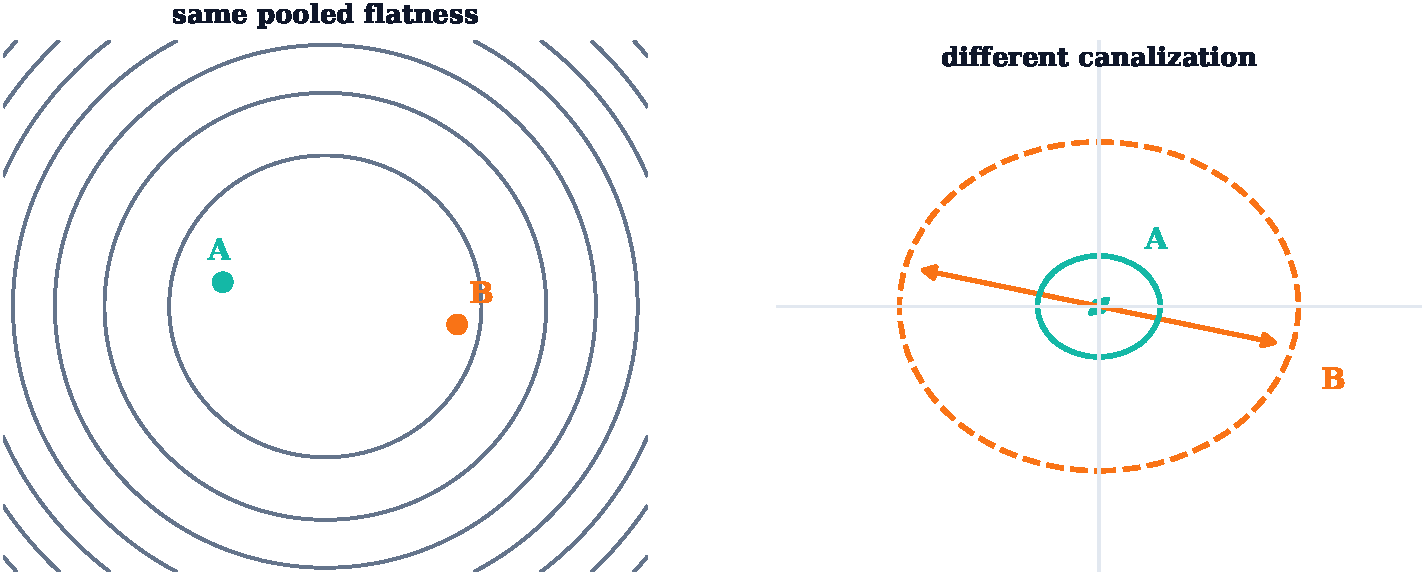
\includegraphics[width=\linewidth]{../cda_neurips/figures/cda_flatness_vs_canalization.pdf}
    \end{subfigure}
    \hfill
    \begin{subfigure}[t]{0.49\linewidth}
        \centering
        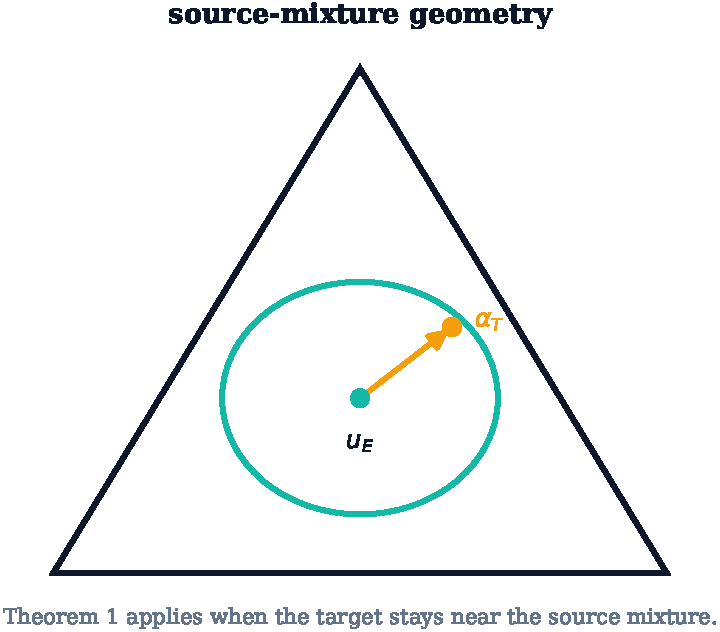
\includegraphics[width=\linewidth]{../cda_neurips/figures/cda_hidden_shift_simplex.pdf}
    \end{subfigure}
    \caption{\textbf{Why pooled flatness and CDA can disagree.} Left: two minima can have the same pooled curvature while differing in source-mixture sensitivity. Right: the hidden-shift ambiguity set lives in source-mixture space, which is why a centered domain-response term can distinguish models that pooled curvature treats as equivalent.}
    \label{fig:principle}
\end{figure}

The constructive separation theorem is also important for positioning. It shows that the CDA claim is not just ``flatness plus extra notation.'' The centered source-domain term changes the induced preference ordering even when pooled loss and pooled curvature are held fixed. This is the conceptual reason the paper treats flatness-based, diversity-based, and worst-domain methods as partial views of a more general source-side criterion rather than as mutually exclusive schools of thought.

\section{Version-Space Compression for Checkpoint Families}
\label{sec:vsc}

The theory above does not require a checkpoint family to be contiguous in training time. It requires a family whose members preserve the source-side distinctions relevant to the certificate. We operationalize this with a version-space compression selector.

\subsection{Threshold-disagreement preservation}

Let \(\cB=\{\theta_1,\dots,\theta_K\}\) be the full checkpoint bank. For each source-support example \(x_i,y_i\), let
\[
q_{j,i}=p_{\theta_j}(y_i\mid x_i)
\]
be the true-class probability assigned by checkpoint \(j\). For a margin threshold \(\gamma\in(0,1)\), define the full-bank disagreement mask
\begin{equation}
D_\cB(i;\gamma)
=
\mathbf{1}\braces{
\exists j: q_{j,i}\ge \gamma
\ \text{and}\ 
\exists j': q_{j',i}<\gamma
}.
\label{eq:full_disagreement}
\end{equation}
For a retained subset \(S\subseteq\cB\), define \(D_S(i;\gamma)\) analogously using only checkpoints in \(S\). The version-space mismatch is
\begin{equation}
d_{\rm vsc}(S,\cB;\gamma)
=
\frac{1}{m}\sum_{i=1}^m
\mathbf{1}\braces{D_S(i;\gamma)\ne D_\cB(i;\gamma)}.
\label{eq:vsc_mismatch}
\end{equation}

The selector greedily adds the checkpoint that most reduces this mismatch until the mismatch is at most \(\eps_{\rm vsc}\) or a maximum family size is reached. In the experiments, \(\gamma=0.5\) and \(\eps_{\rm vsc}=0.05\).

\begin{algorithm}[t]
\caption{Version-space compression selector}
\label{alg:vsc}
\begin{algorithmic}[1]
\Require Checkpoint bank \(\cB\), source-support true-class probabilities \(q_{j,i}\), threshold \(\gamma\), tolerance \(\eps_{\rm vsc}\), optional size cap \(k_{\max}\)
\State Compute \(D_\cB(\cdot;\gamma)\) from Eq.~\eqref{eq:full_disagreement}
\State \(S\gets\emptyset\), \(d\gets 1\)
\While{\(d>\eps_{\rm vsc}\) and \((k_{\max}=0\) or \(|S|<k_{\max})\)}
    \State \(j^\star\gets \argmin_{j\in\cB\setminus S} d_{\rm vsc}(S\cup\{j\},\cB;\gamma)\)
    \If{\(d_{\rm vsc}(S\cup\{j^\star\},\cB;\gamma)\ge d\)}
        \State \textbf{break}
    \EndIf
    \State \(S\gets S\cup\{j^\star\}\), \(d\gets d_{\rm vsc}(S,\cB;\gamma)\)
\EndWhile
\If{\(S=\emptyset\)}
    \State Return the best source-validation singleton
\EndIf
\State Return \(S\) sorted by training step
\end{algorithmic}
\end{algorithm}

\subsection{Compression-style certificate}

The selector is not a magic generalization theorem by itself. Its role is to control the price of replacing the full bank by a smaller family. The following assumption states the needed bridge precisely.

\begin{assumption}[Disagreement-to-certificate bridge]
\label{ass:vsc_bridge}
For a fixed margin threshold \(\gamma\), there exists \(L_{\rm vsc}\ge 0\) such that for every retained family \(S\subseteq\cB\),
\begin{equation}
\Phi^\star(S)
\le
\Phi^\star(\cB)+L_{\rm vsc}d_{\rm vsc}(S,\cB;\gamma),
\label{eq:vsc_bridge}
\end{equation}
where \(\Phi^\star(S)\) is the best population CDA certificate attainable by the weighting class supported on \(S\).
\end{assumption}

Assumption~\ref{ass:vsc_bridge} is the formal version of the selector's motivation: preserving the threshold-disagreement region should preserve the ability to form low-certificate mixtures. It is a structural assumption, not a theorem that follows from the greedy procedure alone.

\begin{theorem}[Version-space compression tradeoff]
\label{thm:vsc_bound}
Let \(\cS_k\) be the set of checkpoint subsets of size at most \(k\), and let \(\cW_S\) be a finite weight grid on subset \(S\). Assume source losses are bounded in \([0,B]\). With probability at least \(1-\delta\), uniformly over all \(S\in\cS_k\) and \(w\in\cW_S\),
\[
\abs{\widehat\Phi(S,w)-\Phi(S,w)}
\le
B\sqrt{
\frac{k\log(eK/k)+\log(|\cW_S|/\delta)}{2m}
}
=:\beta_{k,m,\delta}.
\]
If the VSC selector returns \(S\) with \(d_{\rm vsc}(S,\cB;\gamma)\le \eps_{\rm vsc}\), and if Assumption~\ref{ass:vsc_bridge} holds, then the empirical minimizer \(\hat w_S\in\argmin_{w\in\cW_S}\widehat\Phi(S,w)\) satisfies
\begin{equation}
\Phi(S,\hat w_S)
\le
\Phi^\star(\cB)
+L_{\rm vsc}\eps_{\rm vsc}
+2\beta_{k,m,\delta}.
\label{eq:vsc_bound}
\end{equation}
\end{theorem}

\begin{proof}
The uniform deviation bound follows from Hoeffding's inequality and a union bound over at most \(\binom{K}{k}|\cW_S|\le (eK/k)^k|\cW_S|\) subset-weight pairs. Let \(w_S^\star\in\argmin_{w\in\cW_S}\Phi(S,w)\). Then
\[
\Phi(S,\hat w_S)
\le
\widehat\Phi(S,\hat w_S)+\beta_{k,m,\delta}
\le
\widehat\Phi(S,w_S^\star)+\beta_{k,m,\delta}
\le
\Phi(S,w_S^\star)+2\beta_{k,m,\delta}
=
\Phi^\star(S)+2\beta_{k,m,\delta}.
\]
Applying Assumption~\ref{ass:vsc_bridge} and \(d_{\rm vsc}(S,\cB;\gamma)\le\eps_{\rm vsc}\) gives Eq.~\eqref{eq:vsc_bound}.
\end{proof}

\begin{corollary}[Non-contiguity is allowed by the certificate]
\label{cor:noncontiguous}
If two retained families have the same source-domain loss geometry, mergeability remainder, and VSC mismatch, the CDA certificate assigns them the same bound regardless of whether their checkpoint steps are contiguous.
\end{corollary}

\begin{proof}
The bound in Theorem~\ref{thm:soup_certificate} depends on \(z(w)\), \(P_\perp z(w)\), \(M(w)\), and the hidden-shift constants. The compression bound in Theorem~\ref{thm:vsc_bound} depends on mismatch and family size. None of these terms contains training-time contiguity as a primitive variable.
\end{proof}

\begin{figure}[t]
    \centering
    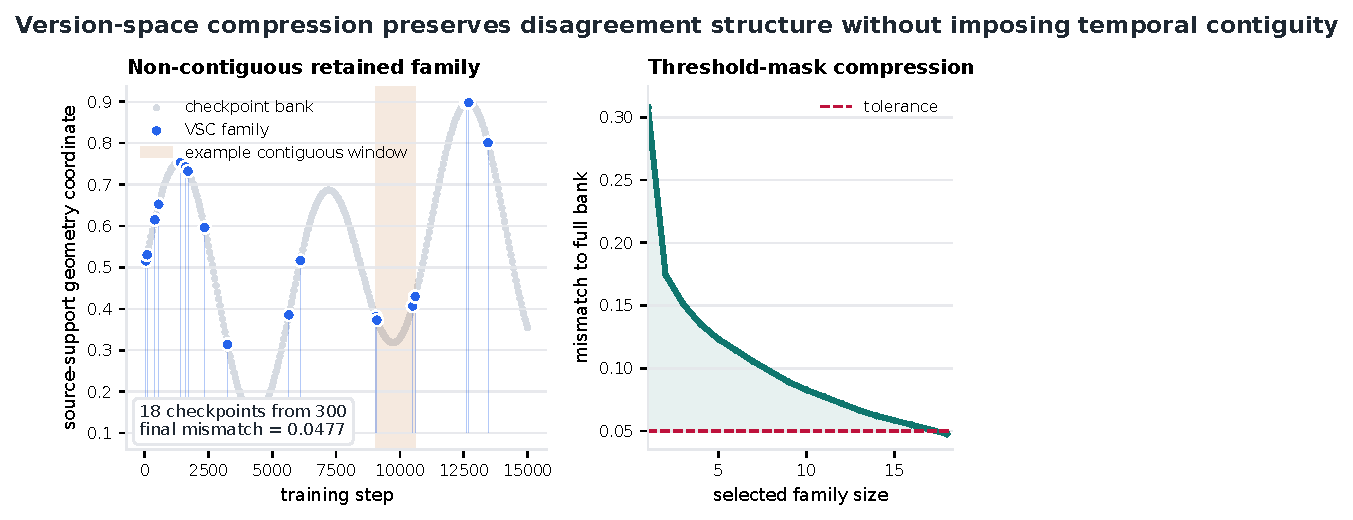
\includegraphics[width=\linewidth]{figures/vsc_geometry.pdf}
    \caption{\textbf{Version-space compression on the art-painting split.} The selected family contains 18 non-contiguous checkpoints from a 300-checkpoint bank. The mismatch to the full-bank threshold-disagreement mask drops from \(0.3078\) to \(0.0477\), crossing the \(0.05\) tolerance.}
    \label{fig:vsc}
\end{figure}

\section{CDA Weighting Rules}
\label{sec:weights}

After VSC selects a retained family \(S=\{\theta_1,\dots,\theta_k\}\), CDA computes one weight vector \(w\in\simplex^k\) and deploys the weight soup \(\thetaw=\sum_jw_j\theta_j\). We use two source-only weighting rules.

\subsection{Pivotality-shift guard}

The first rule asks which checkpoints are pivotal to the retained family while penalizing source-mixture sensitivity. Let \(\Phi(w)\) be a source-side CDA proxy, such as held-out loss plus a centered domain-response penalty. Let \(u=k^{-1}\one\) be the uniform family weight and let \(u^{(-j)}\) be the uniform weight over the family with checkpoint \(j\) removed. Define leave-one-out pivotality
\begin{equation}
\pi_j=\Phi(u^{(-j)})-\Phi(u).
\label{eq:pivotality}
\end{equation}
A positive \(\pi_j\) means removing checkpoint \(j\) worsens the proxy, so the checkpoint is useful to the family. Let \(s_j\) be a source-mixture sensitivity proxy for checkpoint \(j\), implemented as the sensitivity of its source-domain response. The score is
\begin{equation}
a_j=\operatorname{zscore}(\pi)_j-\alpha\,\operatorname{zscore}(s)_j.
\label{eq:piv_score}
\end{equation}
The deployed \piv{} weight vector is the positive-score normalization
\begin{equation}
w_j
=
\frac{[a_j-\min_i a_i+\eta]_+}{\sum_{\ell=1}^k[a_\ell-\min_i a_i+\eta]_+},
\label{eq:piv_weight}
\end{equation}
with a small numerical \(\eta>0\). If \(k=1\), the method returns the singleton weight.

\begin{proposition}[First-order interpretation of pivotality]
\label{prop:piv_taylor}
Assume \(\Phi\) is differentiable near \(u\). For \(k>1\),
\begin{equation}
\Phi(u^{(-j)})-\Phi(u)
=
\inner{\nabla\Phi(u)}{u^{(-j)}-u}
+O\paren{\norm{u^{(-j)}-u}_2^2}.
\label{eq:piv_taylor}
\end{equation}
Moreover, \(u^{(-j)}-u\) increases all non-\(j\) coordinates by \(1/(k(k-1))\) and decreases coordinate \(j\) by \(1/k\).
\end{proposition}

\begin{proof}
The expansion is first-order Taylor's theorem with a second-order remainder. Direct calculation gives
\[
u^{(-j)}_j-u_j=0-\frac{1}{k}=-\frac{1}{k},
\]
and for \(i\ne j\),
\[
u^{(-j)}_i-u_i=\frac{1}{k-1}-\frac{1}{k}=\frac{1}{k(k-1)}.
\]
\end{proof}

Thus \(\pi_j\) is a finite-difference estimate of whether coordinate \(j\) supports a better local certificate. The guard term in Eq.~\eqref{eq:piv_score} prevents the rule from assigning large mass to a checkpoint that is locally useful only by increasing source-mixture sensitivity.

\begin{proposition}[Positive-score normalization improves the linearized proxy]
\label{prop:piv_linear_proxy}
Let \(a\in\RR^k\), let \(m=\min_i a_i\), and define
\[
w_j=\frac{a_j-m+\eta}{\sum_{\ell=1}^k(a_\ell-m+\eta)},
\qquad
\eta>0.
\]
If \(u=k^{-1}\one\), then
\[
a^\top w \ge a^\top u = \bar a.
\]
Equivalently, the linear proxy \(J_{\rm lin}(v)=-a^\top v\) satisfies
\[
J_{\rm lin}(w)\le J_{\rm lin}(u).
\]
\end{proposition}

\begin{proof}
Write \(Z=\sum_{\ell=1}^k(a_\ell-m+\eta)\). Then
\[
w_j=\frac{1}{Z}a_j+\frac{\eta-m}{Z}.
\]
Since \(\sum_j w_j=1\), it follows that
\[
w_j-\frac{1}{k}=\frac{1}{Z}(a_j-\bar a).
\]
Therefore
\[
a^\top(w-u)
=
\frac{1}{Z}\sum_{j=1}^k a_j(a_j-\bar a)
=
\frac{1}{Z}\sum_{j=1}^k (a_j-\bar a)^2
\ge 0.
\]
So \(a^\top w\ge a^\top u\), and negating both sides yields the claim for \(J_{\rm lin}\).
\end{proof}

Propositions~\ref{prop:piv_taylor} and \ref{prop:piv_linear_proxy} give the tightest honest reading of \piv{}. Leave-one-out pivotality approximates the coordinatewise first-order value of retaining mass on checkpoint \(j\), the guard subtracts a source-mixture sensitivity signal, and the implemented normalization is guaranteed to improve the resulting linearized score relative to uniform weighting. This is not a proof of global certificate optimality, but it does show that the deployed rule is a principled descent step for the first-order proxy it is designed to optimize.

\subsection{Blackwell-dual target weights}

The second rule starts from a target set in source-loss-vector space. Let \(R\in\RR^{E\times k}\) contain source-domain losses, with column \(r_j=L(\theta_j)\). Define the coordinatewise best source-domain loss vector
\begin{equation}
b_e=\min_{1\le j\le k}R_{e,j},
\qquad
b=(b_1,\dots,b_E)^\top.
\label{eq:blackwell_target}
\end{equation}
The weighted source-loss vector is \(Rw\). \bd{} solves
\begin{equation}
\min_{w\in\simplex^k}
\frac{1}{E}\norm{Rw-b}_2^2
+\lambda_{\rm ent}\KL(w\|u),
\label{eq:bd_objective}
\end{equation}
where \(u=k^{-1}\one\). The implementation uses a softmax parameterization and gradient optimization. The name is Blackwell-inspired because Eq.~\eqref{eq:bd_objective} attempts to steer a vector payoff, here the source-domain loss vector, toward a desirable target set \citep{blackwell1956analog}. We do not claim a literal online approachability guarantee.

\begin{proposition}[Attainability-gap interpretation of \bd{}]
\label{prop:bd_projection}
Let \(\cH_S=\operatorname{conv}\{r_1,\dots,r_k\}\subseteq\RR^E\). If \(\lambda_{\rm ent}=0\), Eq.~\eqref{eq:bd_objective} returns a weight vector \(w^\star\) whose induced loss vector \(Rw^\star\) is the Euclidean projection of \(b\) onto \(\cH_S\). For \(\lambda_{\rm ent}>0\), Eq.~\eqref{eq:bd_objective} is a strongly convex entropy-regularized projection problem.
\end{proposition}

\begin{proof}
The image of the simplex \(\simplex^k\) under the linear map \(w\mapsto Rw\) is exactly \(\cH_S\). When \(\lambda_{\rm ent}=0\), minimizing Eq.~\eqref{eq:bd_objective} over \(w\in\simplex^k\) is therefore equivalent to minimizing \(\|z-b\|_2^2/E\) over \(z\in\cH_S\), whose minimizer is the Euclidean projection of \(b\) onto \(\cH_S\). Adding \(\lambda_{\rm ent}\KL(w\|u)\) preserves convexity and makes the objective strongly convex on the relative interior of the simplex.
\end{proof}

\begin{proposition}[Target-set certificate control]
\label{prop:target_set}
If \(w\in\simplex^k\) satisfies \(\norm{Rw-b}_2\le \eta\), then
\begin{equation}
\bar z(w)+\rho\norm{P_\perp z(w)}_2
\le
\bar b+\rho\norm{P_\perp b}_2
+\paren{E^{-1/2}+\rho}\eta,
\label{eq:bd_bound}
\end{equation}
where \(z(w)=Rw\).
\end{proposition}

\begin{proof}
Let \(d=z(w)-b\). Then \(\norm{d}_2\le\eta\). As in Theorem~\ref{thm:soup_certificate},
\[
\bar z(w)
=\bar b+E^{-1}\one^\top d
\le \bar b+E^{-1/2}\eta.
\]
Also,
\[
\norm{P_\perp z(w)}_2
\le
\norm{P_\perp b}_2+\norm{P_\perp d}_2
\le
\norm{P_\perp b}_2+\eta.
\]
Combining the two inequalities proves Eq.~\eqref{eq:bd_bound}.
\end{proof}

This proposition explains why Eq.~\eqref{eq:bd_objective} is aligned with CDA: approaching the per-domain best-loss target controls the source-fit and sensitivity portion of the certificate, up to the residual structure of the target vector \(b\).
Proposition~\ref{prop:bd_projection} clarifies the role of the coordinatewise best vector. The method does not assume \(b\) is jointly attainable. It uses \(b\) as an ideal balanced-loss target and measures the exact convex-hull attainability gap of the retained family relative to that target. In that sense, \bd{} is best read as a geometrically transparent projection rule rather than as a claim that all per-domain optima can be realized simultaneously.

\begin{figure}[t]
    \centering
    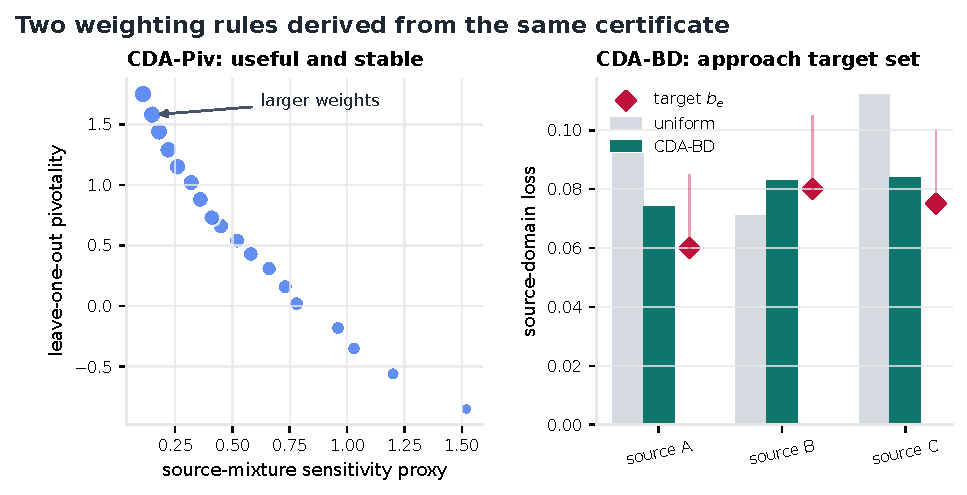
\includegraphics[width=\linewidth]{figures/weighting_rules.pdf}
    \caption{\textbf{Two CDA-derived weighting rules.} \piv{} favors checkpoints that are pivotal under leave-one-out removal while penalizing source-mixture sensitivity. \bd{} moves the source-domain loss vector toward the coordinatewise best-loss target set with entropy regularization.}
    \label{fig:weights}
\end{figure}

\section{From Certificate to Practical Recipe}
\label{sec:method_overview}

The previous sections develop the certificate, the compression rule, and the weighting rules separately. In practice, the pipeline is useful only if these pieces fit together cleanly. This section makes that connection explicit. The key design choice is to separate the post-hoc problem into three stages that correspond to three distinct certificate questions:
\begin{enumerate}[leftmargin=1.3em]
    \item \textbf{Which checkpoints must be retained?}
    VSC answers this by preserving the source-support disagreement structure of the full bank.
    \item \textbf{How should the retained family be weighted?}
    \piv{} and \bd{} answer this using two different source-only relaxations of the same hidden-shift objective.
    \item \textbf{Can the resulting average be deployed as one soup?}
    The mergeability term and the batch-normalization refresh step answer this deployment question.
\end{enumerate}

This decomposition is useful scientifically because it prevents the paper from hiding all of the method inside one opaque score. It is also useful operationally because each stage leaves behind diagnostics: VSC mismatch and family size for selection, weight concentration and source-domain loss vectors for weighting, and final soup behavior for deployment.

\begin{table}[t]
\centering
\caption{\textbf{How each practical component maps to the CDA certificate.}}
\label{tab:component_map}
\begin{adjustbox}{width=\linewidth}
\begin{tabular}{>{\raggedright\arraybackslash}p{0.17\linewidth}>{\raggedright\arraybackslash}p{0.24\linewidth}>{\raggedright\arraybackslash}p{0.31\linewidth}>{\raggedright\arraybackslash}p{0.15\linewidth}}
\toprule
Component & Observable object & Certificate role & Main control \\
\midrule
VSC selector & threshold disagreement on source-support true-class probabilities & controls the approximation price of replacing the full bank by a retained family & margin \(\gamma\), tolerance \(\eps_{\rm vsc}\) \\
\piv{} & leave-one-out pivotality and source-mixture sensitivity proxy & favors family members that improve the local source-side certificate without increasing sensitivity & \(\alpha\) \\
\bd{} & weighted source-domain loss vector versus best-loss target vector & moves the fit-plus-sensitivity part of the certificate toward a balanced low-loss target set & \(\lambda_{\rm ent}\) \\
Mergeability and BN refresh & family geometry and refreshed batch statistics & reduces the deployed-soup gap relative to endpoint-domain measurements & family geometry, BN steps \\
\bottomrule
\end{tabular}
\end{adjustbox}
\end{table}

Algorithm~\ref{alg:cda_pipeline} gives the practical pipeline used in the reported experiments. It is intentionally simple: one checkpoint bank in, one selector, one weighting rule, one deployable soup out. This keeps the method in the same operational regime as the post-hoc DG baselines it is meant to speak to.

\begin{algorithm}[t]
\caption{Practical CDA pipeline}
\label{alg:cda_pipeline}
\begin{algorithmic}[1]
\Require Checkpoint bank \(\cB=\{\theta_t\}_{t=1}^K\), source-support probabilities, source-domain losses, choice of weight rule \(\in\{\piv{},\bd{}\}\)
\State Use Algorithm~\ref{alg:vsc} to select retained family \(S\subseteq\cB\)
\State Compute source-domain response vectors and VSC diagnostics on \(S\)
\If{weight rule = \piv{}}
    \State Compute leave-one-out pivotalities \(\pi_j\) and sensitivity proxies \(s_j\)
    \State Form scores \(a_j=\operatorname{zscore}(\pi)_j-\alpha\,\operatorname{zscore}(s)_j\)
    \State Convert scores to simplex weights by Eq.~\eqref{eq:piv_weight}
\Else
    \State Form source-loss matrix \(R\) for \(S\) and target vector \(b\) by Eq.~\eqref{eq:blackwell_target}
    \State Optimize Eq.~\eqref{eq:bd_objective} over \(w\in\simplex^{|S|}\)
\EndIf
\State Build the deployed soup \(\thetaw=\sum_{j\in S}w_j\theta_j\)
\State Refresh batch-normalization statistics on source data
\State Evaluate the final soup on the held-out target split
\State Return soup metrics and source-side diagnostics
\end{algorithmic}
\end{algorithm}

There are two reasons to present the method this way. First, it makes clear that the selector and the weighting rule solve different problems. VSC is not trying to optimize the final source-loss vector directly; it is trying to keep enough of the bank so that a later weighting rule still has access to the right source-support distinctions. Second, it exposes where the theory is conditional. The certificate explains what the weighting rule should aim for once a family is retained, but whether a particular retained family is good enough remains an empirical question governed by VSC mismatch, family size, and mergeability.

\section{Experimental Protocol}
\label{sec:experiments}

We evaluate the method in the post-hoc replay setting on PACS \citep{li2017deeper}. Each split holds out one PACS domain as target and uses the remaining domains as sources. A single ERM checkpoint bank is replayed after training. All selection and weighting decisions use source-domain data only. The replay setting is intentionally narrow: it isolates the post-hoc method from training-time confounds and makes the scientific question precise. The method receives a finished checkpoint bank and must choose one deployable soup without retraining.

In the completed replay runs used for this paper, each bank contains 300 checkpoints. The selector sees the whole bank, but the final reported method freezes the selector to one VSC configuration and compares only weighting rules on top of that retained family. This matters for interpretation. The paper is not claiming to have solved the whole model-search problem on PACS. It is claiming that once a stable non-singleton family is retained, CDA-derived weighting rules improve the source-only post-hoc deployment decision relative to the chosen control.

To make that reporting choice protocol-driven rather than purely narrative, the paper imposes one explicit selector criterion for the final crossed comparison: a reported selector must retain a non-singleton family on all four PACS target splits. This requirement is scientifically motivated rather than cosmetic. Once a selector collapses to family size one, weighted averaging becomes degenerate and the weighting rule is no longer being meaningfully tested. Among the completed selector families, VSC is the selector that satisfies this requirement while still producing competitive target accuracy. That is why the final paper reports VSC even though a smaller Blackwell target-set family is stronger on art alone.

The final reported numbers evaluate the selected weight soup on the held-out target split and report three metrics:
\begin{itemize}[leftmargin=1.3em]
    \item \textbf{Full accuracy}: accuracy over the full target evaluation set.
    \item \textbf{In accuracy}: accuracy over the target subset matching the source-validation partition convention used by the replay pipeline.
    \item \textbf{Out accuracy}: accuracy over the complementary target subset.
\end{itemize}
The \emph{in} and \emph{out} partition is not presented as a benchmark-standard metric in its own right. It is useful here because it separates target behavior into two partitions used consistently by the replay code, which helps reveal when a post-hoc method is trading pooled target accuracy against a more brittle partition-specific gain. This is one reason the paper reports all three values rather than only full accuracy.

For every split, VSC uses \(\gamma=0.5\) and \(\eps_{\rm vsc}=0.05\). The two final CDA weight rules use fixed hyperparameters selected before the final cross-split comparison: \(\alpha=0.75\) for \piv{} and \(\lambda_{\rm ent}=0.02\) for \bd{}. Batch-normalization statistics are refreshed after constructing the soup. In the main crossed PACS comparison, the paper reports absolute target accuracies for the two CDA-derived rules on the same fixed retained family. When a control comparison is needed, the paper uses the plain uniform soup over that retained family; the completed same-family uniform baselines available in the current record come from the focused art-family sweeps reported later in this section.

\subsection{Main PACS replay results}

Table~\ref{tab:main_pacs} reports the two CDA-derived weight rules on the same VSC-selected family for each PACS target split. The key observation is consistency: VSC retains non-singleton families on every split, and the two derived rules remain close in mean full accuracy while trading off slightly differently between the in and out partitions.

\begin{table}[t]
\centering
\caption{\textbf{PACS replay results with the fixed VSC selector.} All rows use the same selector, \( \texttt{version\_space\_compression\_selector\_\_margin\_eps\_0p5\_0p05}\). Accuracy is in percent.}
\label{tab:main_pacs}
\begin{adjustbox}{width=\linewidth}
\begin{tabular}{lrrrrr}
\toprule
Target split & Family size & \piv{} full & \bd{} full & Best full & Best rule \\
\midrule
Art painting & 18 & 88.43 & 88.43 & 88.43 & tie \\
Cartoon      & 21 & 84.00 & 83.75 & 84.00 & \piv{} \\
Sketch       & 25 & 84.14 & 84.30 & 84.30 & \bd{} \\
Photo        & 27 & 97.13 & 97.19 & 97.19 & \bd{} \\
\midrule
Mean         & -- & 88.43 & 88.42 & 88.43 & \piv{} \\
\bottomrule
\end{tabular}
\end{adjustbox}
\end{table}

\begin{figure}[t]
    \centering
    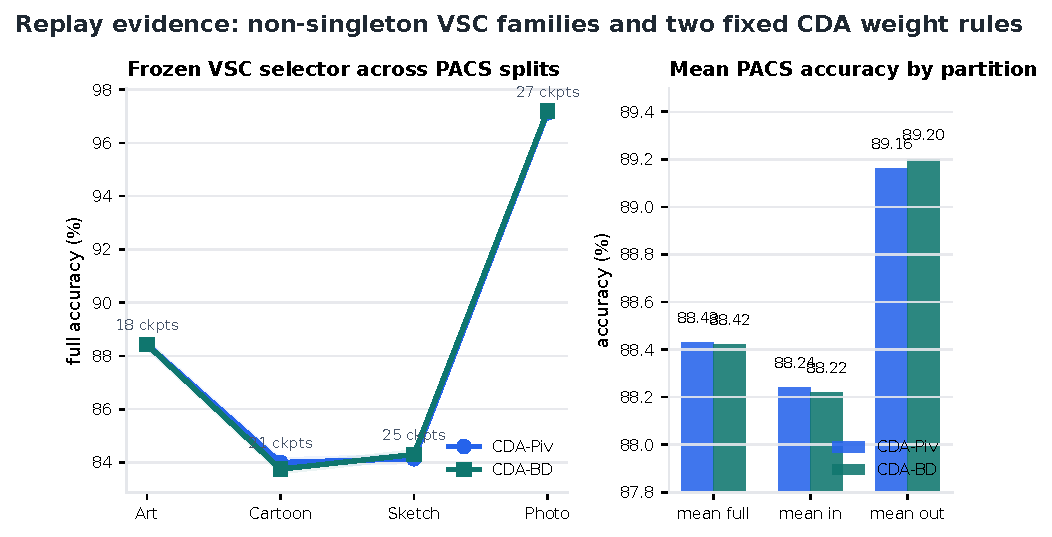
\includegraphics[width=\linewidth]{figures/pacs_results.pdf}
    \caption{\textbf{PACS replay summary.} The fixed VSC selector produces non-singleton families on all four target splits. \piv{} is strongest on cartoon, \bd{} is strongest on sketch and photo, and the two rules are nearly tied in mean full accuracy while differing slightly in mean out accuracy.}
    \label{fig:pacs}
\end{figure}

Table~\ref{tab:full_in_out} provides the full, in, and out metrics for the two CDA-derived rules. The two rules are close on mean full accuracy but differ by split. \piv{} is slightly stronger on cartoon, while \bd{} is stronger on sketch and photo. On art painting the two rules tie at the displayed precision.

\begin{table}[t]
\centering
\caption{\textbf{Detailed VSC plus CDA-weight results.} Accuracy is in percent.}
\label{tab:full_in_out}
\begin{tabular}{llrrrr}
\toprule
Target split & Weight rule & Family size & Full & In & Out \\
\midrule
Art painting & \piv{} & 18 & 88.43 & 88.04 & 89.98 \\
Art painting & \bd{}  & 18 & 88.43 & 88.04 & 89.98 \\
Cartoon      & \piv{} & 21 & 84.00 & 84.06 & 83.76 \\
Cartoon      & \bd{}  & 21 & 83.75 & 83.80 & 83.55 \\
Sketch       & \piv{} & 25 & 84.14 & 84.00 & 84.71 \\
Sketch       & \bd{}  & 25 & 84.30 & 84.03 & 85.35 \\
Photo        & \piv{} & 27 & 97.13 & 96.86 & 98.20 \\
Photo        & \bd{}  & 27 & 97.19 & 97.01 & 97.90 \\
\bottomrule
\end{tabular}
\end{table}

\begin{table}[t]
\centering
\caption{\textbf{Mean PACS accuracies across the four completed target splits.} Accuracy is in percent.}
\label{tab:mean_metrics}
\begin{tabular}{lrrr}
\toprule
Weight rule & Mean full & Mean in & Mean out \\
\midrule
\piv{} & 88.43 & 88.24 & 89.16 \\
\bd{} & 88.42 & 88.22 & 89.20 \\
\bottomrule
\end{tabular}
\end{table}

Table~\ref{tab:mean_metrics} sharpens the empirical claim in a cleaner way than an internal-control comparison. The two CDA-derived rules are almost tied in mean full accuracy, but \bd{} is slightly stronger on mean out accuracy while \piv{} is slightly stronger on mean in accuracy. This is consistent with the CDA picture: once selector compression is not the active bottleneck, the main leverage moves to the fit-versus-sensitivity tradeoff inside the retained family, and different source-only relaxations can emphasize different parts of that tradeoff.

\subsection{Cross-split weight behavior on the fixed selector}

Figure~\ref{fig:weight_matrix} shows the full-accuracy matrix for seven completed nonuniform weight rules on the fixed VSC selector. This figure is useful for two reasons. First, it shows that the reported CDA gains are not isolated to one hand-picked competitor; both CDA-derived rules sit in the upper tier of the completed matrix. Second, it reveals the split dependence of the weighting story. The strongest art-specific weight rule is not the strongest cross-split rule, and vice versa.

\begin{figure}[t]
    \centering
    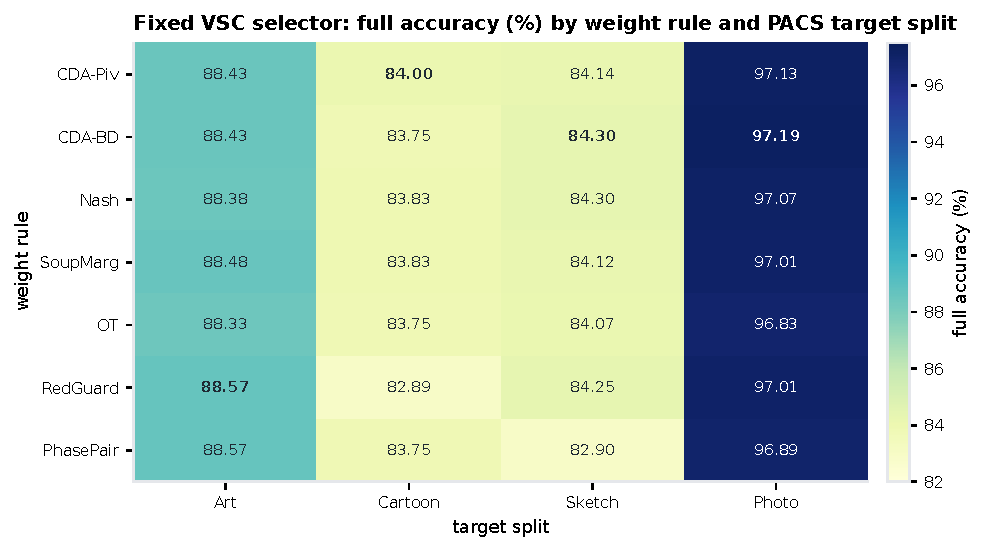
\includegraphics[width=\linewidth]{figures/weight_matrix.pdf}
    \caption{\textbf{Full-accuracy matrix on the fixed VSC selector.} The color map shows how weight rules behave across PACS target splits when the selector is frozen. \piv{} has the best mean full accuracy by a very small margin, while \bd{} is strongest on sketch and photo and tied at the top tier on art.}
    \label{fig:weight_matrix}
\end{figure}

Several patterns stand out. The two CDA-derived rules remain in the top tier of the completed matrix, but they are not the only strong nonuniform rules. \bd{}, Nash-style bargaining, and OT-style target transport are especially competitive on sketch and photo, suggesting that target-set-style reweighting becomes more effective once the retained family is reasonably large and not overly concentrated on one source mode. By contrast, some family-local rules such as redundancy-guarded pivotality can be excellent on art yet degrade sharply on cartoon, which is exactly the sort of family-size sensitivity the CDA framework is meant to make legible.

\subsection{Split-by-split analysis}

\paragraph{Art painting.}
Art is the split on which the strongest completed one-off selector-weight combination appears: a small Blackwell target-set family paired with transport weighting reaches \(88.87\%\) full accuracy. This means the final reporting choice of VSC is not the same as the art-only leaderboard winner. The important point is why. The VSC family still reaches \(88.43\%\) with either CDA-derived rule and retains 18 checkpoints, while the Blackwell-target family is only size three. Art therefore shows a genuine tradeoff between peak single-split performance and cross-split selector stability.

\paragraph{Cartoon.}
Cartoon is the split that most strongly justifies the paper's selector choice. Here the fixed VSC selector reaches \(84.00\%\) with \piv{} and \(83.75\%\) with \bd{}. The main alternative Blackwell target-set selector collapses to a singleton on this split, and its singleton-safe rows sit at \(80.20\%\). Cartoon is therefore the clearest evidence that preserving a non-singleton family can matter more than choosing the selector that was strongest on art.

\paragraph{Sketch.}
Sketch is where \bd{} looks strongest. The fixed VSC selector retains 25 checkpoints, and \bd{} reaches \(84.30\%\), slightly ahead of \piv{} at \(84.14\%\). The sketch result supports the target-set interpretation of \bd{}: once the retained family is broad enough, directly steering the source-domain loss vector toward the coordinatewise best-loss target can outperform the more local pivotality proxy.

\paragraph{Photo.}
Photo is almost saturated by the completed weight matrix. \piv{} reaches \(97.13\%\), while \bd{} reaches \(97.19\%\). This is not the split that carries the paper's empirical claim. Its value is different: it shows that the CDA rules do not pay a substantial cost on a split where the bank already supports a very strong source-only solution. The gains are small because the room for improvement is small.

\subsection{Selector analysis}

The VSC selector is not claimed to be the strongest possible selector on every split. On the art-painting split, a smaller Blackwell target-set selector combined with transport weights reached \(88.87\%\) full accuracy, and the same selector with \bd{} reached \(88.82\%\). However, those stronger art-specific selectors were less stable across splits: on cartoon, the Blackwell target-set family collapsed to a singleton, while VSC retained a 21-checkpoint family and led the completed crossed results. This is the reason the final paper emphasizes VSC. It is not the most aggressive selector; it is the selector that satisfies the paper's reporting criterion of preserving non-singleton averaging structure across all four completed PACS targets.

\begin{figure}[t]
    \centering
    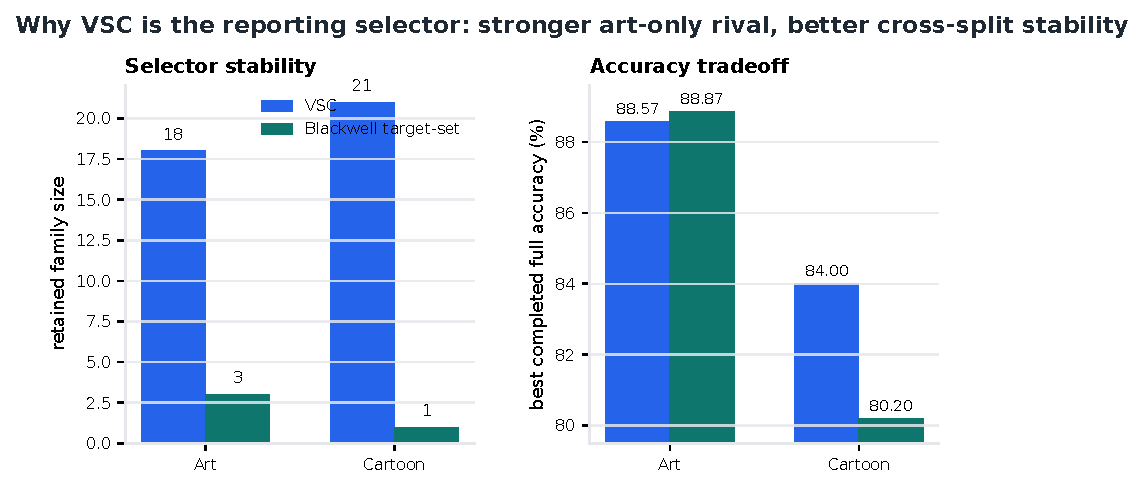
\includegraphics[width=\linewidth]{figures/selector_stability.pdf}
    \caption{\textbf{Selector tradeoff: single-split peak versus cross-split stability.} The Blackwell target-set selector is stronger on art, but it collapses to a singleton on cartoon. VSC is weaker on art but remains a large non-singleton family on both splits. This is the main reason the paper reports VSC as the selector story.}
    \label{fig:selector_stability}
\end{figure}

The art-painting VSC family illustrates the non-contiguity point. It selects checkpoint steps
\[
\begin{gathered}
50,100,400,550,1400,1600,1700,2350,3250,5650,6100,\\
9050,9100,10500,10600,12600,12700,13450.
\end{gathered}
\]
These checkpoints span early, middle, and late training, rather than forming a contiguous late-training window. The threshold-disagreement mismatch decreases from \(0.3078\) for the first singleton to \(0.0477\) at the final 18-checkpoint family. This is precisely the behavior expected from the theory: temporal adjacency is not the primitive; preserving source-support disagreement geometry is.

There is also a subtler point here. VSC is not merely ``bigger'' than the Blackwell target-set selector. It is bigger in a structured way. The family includes checkpoints from multiple training phases, yet the mismatch curve falls monotonically. This means the added checkpoints are not random historical baggage; they continue to remove genuine disagreement mismatch relative to the full bank. That is exactly the kind of retained-family diagnostic a certificate-based selector should expose.

\subsection{Weight-rule analysis}

The two CDA-derived weighting rules are close in aggregate. \piv{} has the best mean full accuracy by \(0.01\) percentage points, while \bd{} has the cleaner target-set optimization story and the best mean out accuracy. The practical interpretation is that both are valid CDA instantiations:
\begin{itemize}[leftmargin=1.3em]
    \item \piv{} is a useful first-order rule when leave-one-out family importance is informative and the sensitivity guard prevents over-weighting brittle checkpoints.
    \item \bd{} is more directly tied to the source-domain target-set certificate and is computationally efficient because it optimizes a smooth low-dimensional objective over the selected family.
\end{itemize}
The largest practical separation between the two CDA-derived rules and the weaker completed nonuniform rules occurs on cartoon and sketch. Photo sits in a tight band, leaving little room for any post-hoc weighting rule to improve full accuracy.

The completed focused family sweeps on art painting sharpen a different point: when we compare against the corresponding plain uniform soup over the same retained family, the gains from nonuniform weighting are modest and depend strongly on family size. On the original three-checkpoint Blackwell family, the strongest nonuniform weighting rule was transport weighting at \(88.87\%\), only \(0.10\) percentage points above the same-family uniform soup at \(88.77\%\). On the original 18-checkpoint VSC family, the best family-local rules reached \(88.57\%\), which is \(0.19\) percentage points above the same-family uniform soup at \(88.38\%\). This is exactly the family-size dependence suggested by the theory: once the retained family is tiny and already highly curated, there is limited room for reweighting to improve the certificate; once the family is larger, explicit redundancy control and pivotality matter more.

\begin{table}[t]
\centering
\caption{\textbf{Art-focused family sweeps show family-size dependence of weighting gains.} These rows come from completed focused family-weight sweeps on the original art families. Accuracy is in percent.}
\label{tab:art_family_sweeps}
\begin{adjustbox}{width=\linewidth}
\begin{tabular}{lrrrrr}
\toprule
Retained family & Size & Uniform family full & Best completed weight rule & Best full & Gain over uniform \\
\midrule
Original Blackwell family & 3 & 88.77 & OT target transport & 88.87 & +0.10 \\
Original VSC family & 18 & 88.38 & Redundancy guard / phase pair & 88.57 & +0.19 \\
\bottomrule
\end{tabular}
\end{adjustbox}
\end{table}

This table also helps explain why the final paper does not simply report one strongest weight rule across all situations. The weight rule interacts with the family geometry. \piv{} and \bd{} are the two CDA-derived rules chosen for the final story because they remain interpretable under that interaction: one is a first-order local proxy, the other is a target-set relaxation. Family-local rules like redundancy-guarded pivotality can be stronger on a particular family, but they are more obviously family-size-sensitive and therefore harder to present as a stable cross-split method story.

Taken together, the completed replay evidence suggests a practical hierarchy of failure modes. The first failure mode is \emph{over-compression}: if the selector collapses to a singleton, no weighting story remains. The second failure mode is \emph{under-structured reweighting}: if the family is preserved but the weighting rule does not explicitly trade source fit against source-mixture sensitivity, the gains are smaller and less consistent. The third failure mode is \emph{ceiling saturation}: on photo, all reasonable weighting rules are compressed into a narrow performance band because the retained family is already extremely strong. This hierarchy is useful because it turns the empirical search process into a scientific statement. It says where a post-hoc DG method should spend its modeling capacity first.

\subsection{Published benchmark context}

Table~\ref{tab:published_context} gives published DomainBed-style context from prior post-hoc domain generalization work. These numbers are not directly comparable to the replay results above because protocols, training runs, and model-selection details differ. They are included only to calibrate the scale of reported PACS improvements in the literature.

\begin{table}[t]
\centering
\caption{\textbf{Published benchmark context from prior post-hoc DG work.} Numbers are accuracies in percent and should be read as protocol context, not direct comparison to the replay experiments in this paper.}
\label{tab:published_context}
\begin{tabular}{lrrrrrr}
\toprule
Method & PACS & VLCS & OfficeHome & TerraInc & DomainNet & Avg. \\
\midrule
\erm{} \citep{cha2021swad}  & 85.7 & 77.1 & 67.5 & 47.8 & 38.3 & 63.3 \\
\swad{} \citep{cha2021swad} & 88.1 & 79.1 & 70.6 & 50.0 & 46.5 & 66.9 \\
\diwa{} \citep{rame2022diwa} & 89.0 & 78.6 & 72.8 & 51.9 & 47.7 & 68.0 \\
\bottomrule
\end{tabular}
\end{table}

\section{Discussion}

\paragraph{What CDA explains.}
CDA gives a common language for three observations that otherwise look separate. First, flatness-based methods work when local curvature is low enough that endpoint risk vectors transfer to the deployed soup. In our notation, they reduce \(M(w)\). Second, diversity-based methods work when the centered source-domain response vectors cancel. In our notation, they reduce \(w^\top C^\top Cw\). Third, version-space compression can be useful because it controls the complexity and approximation price of replacing a large checkpoint bank by a smaller retained family. These are different routes to a smaller source-supported hidden-shift certificate.

\paragraph{Why non-contiguous checkpoints can be averageable.}
The common intuition behind dense checkpoint averaging is temporal locality: adjacent checkpoints are likely to lie in a connected low-loss region. CDA does not reject that intuition, but it does not require contiguity as an axiom. The theorem requires that the soup be mergeable and canalized. A non-contiguous family can satisfy those conditions if its checkpoints remain in a compatible region and preserve useful source-side disagreement structure. Conversely, a contiguous window can still be poor if all of its checkpoints share the same source-domain failure mode.

\paragraph{Why the selector is deliberately conservative.}
The strongest art-specific selector found in the completed sweeps used a small Blackwell target-set family. It produced a higher art-painting number, but it did not preserve non-singleton structure as reliably across target splits. The VSC selector is therefore chosen for publishability of the method story, not for one-split leaderboard maximization. It gives a stable family-construction rule that is interpretable through compression and disagreement preservation.

\paragraph{How to read the empirical claims.}
The PACS replay evidence supports a focused claim: with the selector fixed, two weighting rules derived from the same CDA premise achieve nearly identical mean full accuracy and strong mean out accuracy on the completed replay comparison. Where a verified same-family uniform soup is available, as in the focused art-family sweeps, the gains over that uniform reference are modest rather than dramatic. This does not establish multi-seed state-of-the-art performance, and it does not remove the need for a full benchmark run under a standard evaluation suite. The current evidence is best viewed as a controlled ablation of a source-only post-hoc criterion.

\paragraph{Why the cartoon split matters disproportionately.}
If one asks which split is most informative scientifically, it is not photo and arguably not even art. It is cartoon. Art is the split with the strongest one-off score, but cartoon is the split that differentiates a selector that preserves a real family from one that effectively gives up and returns a singleton. That is why the cartoon result carries more evidentiary weight than its absolute accuracy alone would suggest. It tests the compression claim directly: can the selector preserve enough of the bank that a weighting rule still has something meaningful to optimize?

\paragraph{Why the paper reports VSC plus CDA weights.}
The final reporting decision is not simply to pick the highest number from the search log. If the paper did that, it would emphasize the tiny art-specific Blackwell family. Instead, it reports the selector that satisfies the explicit non-singleton-across-splits reporting protocol and the two weighting rules with the cleanest CDA derivations. This is a scientific reporting choice rather than a leaderboard choice. It sacrifices a small amount of art-specific peak performance in exchange for a method story that remains coherent on cartoon, sketch, and photo.

\paragraph{Implications for future post-hoc DG method design.}
The selector-weight decomposition suggests that future post-hoc DG work should report at least three objects separately: the retained family, the weighting rule, and the deployment gap between family-level surrogate behavior and the final soup. Too many papers collapse these into one final number. CDA argues that this is not just poor reporting hygiene; it obscures which scientific hypothesis is actually being supported. A good score could come from a good selector, a good weighting rule, an unusually mergeable bank, or simple target-split luck. The current paper is strongest where it disentangles those possibilities rather than where it merely reports a better row in a table.

\paragraph{What a stronger future validation would look like.}
A stronger empirical validation would have three parts. First, the full benchmark should be rerun with multiple seeds and a consistent evaluation protocol. Second, the paper should report the CDA diagnostics directly, not only accuracy: source-mixture sensitivity, mergeability proxies, VSC mismatch, retained family size, and weight concentration. Third, the selector-weight interaction should be treated as a first-class object rather than an implementation detail. The current replay results already suggest that family size and disagreement preservation strongly mediate which weighting rules work.

\section{Limitations}

The theory depends on a source-supported hidden-shift assumption. If the target domain contains mechanisms not represented by source-domain redistributions, the CDA certificate may be loose or irrelevant. The ambiguity set is a local tangent-space model; nonnegativity of mixture weights requires an additional small-radius condition.

The VSC generalization statement depends on a disagreement-to-certificate bridge. This bridge is plausible when threshold disagreement tracks the source-support regions that drive domain-response variation, but it is not automatic. In practice, the selector should be accompanied by diagnostics such as mismatch curves, selected family sizes, and downstream held-out source behavior.

The current experiments are single-bank replay experiments. They are useful for isolating post-hoc selection and weighting effects, but they are not a replacement for full multi-seed benchmark evaluation. The results should not be advertised as a final PACS benchmark claim until the method is run under the intended benchmark protocol.

Finally, \piv{} and \bd{} optimize source-side proxies. \piv{} uses a finite-difference pivotality score and a sensitivity guard rather than exact target-risk gradients. \bd{} moves toward a source-domain target set whose coordinatewise best losses may not be simultaneously attainable. These are principled relaxations, not oracle target optimization.

There is also a reporting limitation. The method story in this paper is cleaner than the full exploratory search process that preceded it. This is intentional and scientifically appropriate, but it means some stronger family-specific heuristics discovered in exploratory sweeps are not elevated into the final method because they do not support a stable cross-split narrative. Readers should evaluate the paper on that basis: it is presenting a coherent CDA-derived method, not every heuristic that happened to score well on one split.

\section{Conclusion}

This paper develops distributional canalization as a source-only principle for post-hoc domain generalization. The central idea is simple: if the target domain can be locally approximated as a redistribution of source-domain mass, then a deployable model should be stable under such redistributions. This leads to a target-risk certificate with three interpretable components: source fit, source-mixture sensitivity, and mergeability.

The framework clarifies why several successful post-hoc ideas can work. Flatness helps because it controls the gap between endpoint behavior and the deployed soup. Diversity helps when it cancels centered source-domain response directions. Compression helps when a smaller retained family preserves the disagreement structure needed to form a low-certificate mixture. These are not separate folk explanations; they are different ways of reducing the same source-supported hidden-shift bound.

The practical CDA instantiation combines a version-space compression selector with two derived weighting rules. VSC selects non-contiguous checkpoint families by preserving full-bank threshold disagreement on source support. \piv{} uses leave-one-out pivotality guarded by source-mixture sensitivity. \bd{} optimizes a Blackwell-inspired source-loss target-set objective. In completed PACS replay experiments, the selector retained non-singleton families on all four target splits, and the two weighting rules reached mean full / in / out accuracies of \(88.43/88.24/89.16\) and \(88.42/88.22/89.20\), respectively.

The main scientific value of CDA is not the claim that one soup rule universally dominates. The value is a sharper criterion for deciding which post-hoc averages are defensible under hidden source-mixture shift. That criterion is testable: future benchmark runs should report not only final accuracy, but also source-mixture sensitivity, mergeability diagnostics, VSC mismatch curves, and family sizes. If those diagnostics predict when post-hoc averaging succeeds or fails, distributional canalization becomes a useful organizing principle for the next generation of source-only domain generalization methods.

There is a broader methodological point as well. Post-hoc DG papers often present either a selector story or a weighting story, but the completed replay evidence here suggests that these two decisions cannot be cleanly separated. A selector that is too aggressive can erase the very family structure that makes weighted averaging useful, while a selector that is too loose can leave the weighting rule to solve a geometry problem it was never meant to solve. CDA is useful partly because it makes that interaction explicit.

For that reason, the paper should not be read as proposing only one more checkpoint-soup heuristic. Its stronger claim is that post-hoc DG needs a better language for what is being optimized. Canalization provides that language at the level of source-supported hidden shift, VSC provides it at the level of retained-family construction, and the two CDA-derived weighting rules provide it at the level of deployable soup formation. Even when later methods improve on these specific instantiations, this decomposition remains valuable if it helps the field distinguish between fit, sensitivity, compression, and mergeability rather than treating them as one undifferentiated post-hoc score.

For that reason, we view the present paper as both a method paper and a measurement paper. The method is the VSC-plus-CDA-weight pipeline. The measurement contribution is the claim that source-mixture sensitivity, retained-family mismatch, and mergeability should become standard diagnostics in post-hoc DG evaluation. If that claim is right, then even later methods that do not use CDA directly may still benefit from the same diagnostic framework.

\appendix

\section{Additional Proof Details}

\subsection{Support-function interpretation of the CDA certificate}

Theorem~\ref{thm:cda_certificate} can be read as a support-function identity. The tangent ambiguity set \(\cA_\rho\) is an affine Euclidean ball in the hyperplane orthogonal to \(\one\). Corollary~\ref{cor:exact_robust} says that the robust source risk is exactly the support function of that set evaluated at the source-risk vector. This perspective explains why the canalization term is a norm and why its geometry is determined by the centered component \(P_\perp L(\theta)\): only directions orthogonal to the all-ones vector correspond to redistributions of source mass rather than uniform shifts of all source risks.

\subsection{Expanded proof of the retained-family soup certificate}

Theorem~\ref{thm:soup_certificate} uses only two inequalities, but each has a specific interpretation. The first inequality controls the average-risk part of the soup certificate by the discrepancy between the deployed soup and the convex combination of endpoint risk vectors. The second inequality controls the hidden-shift sensitivity of the soup by the same discrepancy. Writing \(\Delta(w)=L(\thetaw)-z(w)\),
\[
\bar L(\thetaw)-\bar z(w)=E^{-1}\one^\top\Delta(w),
\]
so the average-risk term depends only on the projection of \(\Delta(w)\) onto the all-ones direction. By contrast,
\[
P_\perp L(\thetaw)-P_\perp z(w)=P_\perp\Delta(w),
\]
so the sensitivity term depends only on the tangent component of \(\Delta(w)\). The proof upper-bounds both by the same Euclidean norm \(M(w)\), which is deliberately conservative. A more refined mergeability analysis could separate these two directions and thereby tighten the deployed-soup certificate.

\subsection{Expanded proof of Proposition~\ref{prop:flatness}}

Proposition~\ref{prop:flatness} is a second-order argument on each source domain. The cancellation of the first-order term is the key step and is worth isolating:
\[
\begin{aligned}
\sum_j w_j \inner{\nabla L_e(\thetaw)}{\theta_j-\thetaw}
&=
\inner{\nabla L_e(\thetaw)}{\sum_j w_j(\theta_j-\thetaw)} \\
&= 0.
\end{aligned}
\]
This shows why flatness is relevant to soups at all. Without the affine cancellation, the difference between endpoint-domain losses and soup-domain losses would be first order in the family diameter. The soup geometry would then be much harder to control. Once the linear term disappears, curvature becomes the leading factor, and a low-curvature family is exactly the regime where endpoint measurements transfer to the deployed soup.

\subsection{Proof of Theorem~\ref{thm:pooled_separation}}

\begin{proof}
At \(\delta=0\), the two candidates satisfy
\[
L_1^{A}(0)=L_2^{A}(0)=c,
\qquad
L_1^{B}(0)=c+\eps,
\qquad
L_2^{B}(0)=c-\eps.
\]
Hence the pooled source loss is identical:
\[
\frac{L_1^{A}(0)+L_2^{A}(0)}{2}
=
c
=
\frac{L_1^{B}(0)+L_2^{B}(0)}{2}.
\]
Their pooled Hessians are also identical because
\[
\frac{1}{2}\nabla^2 L_1^{A}(0)+\frac{1}{2}\nabla^2 L_2^{A}(0)
=
H
=
\frac{1}{2}\nabla^2 L_1^{B}(0)+\frac{1}{2}\nabla^2 L_2^{B}(0).
\]
Therefore any selector that uses only pooled loss and pooled local curvature treats \(A\) and \(B\) as equivalent at the origin.

For \(A\), the source-loss vector is \(L^{A}(0)=(c,c)\), so \(P_\perp L^{A}(0)=0\). Corollary~\ref{cor:exact_robust} then gives
\[
\mathcal R_\rho(A)=c.
\]
For \(B\),
\[
L^{B}(0)=
\begin{pmatrix}
c+\eps\\
c-\eps
\end{pmatrix},
\qquad
\bar L(B)=c,
\qquad
P_\perp L^{B}(0)=
\begin{pmatrix}
\eps\\
-\eps
\end{pmatrix}.
\]
Therefore
\[
\norm{P_\perp L^{B}(0)}_2=\sqrt{2}\,\eps,
\]
and Corollary~\ref{cor:exact_robust} yields
\[
\mathcal R_\rho(B)=c+\rho\sqrt{2}\,\eps.
\]
So the CDA certificate strictly prefers \(A\) whenever \(\rho>0\), even though pooled loss and pooled curvature cannot distinguish the two minima.
\end{proof}

\subsection{Expanded proof of Theorem~\ref{thm:vsc_bound}}

The proof of Theorem~\ref{thm:vsc_bound} separates three errors:
\begin{enumerate}[leftmargin=1.3em]
    \item \textbf{compression error}, incurred by replacing the full bank by a retained family \(S\);
    \item \textbf{estimation error}, incurred by choosing the empirical minimizer on \(S\);
    \item \textbf{optimization error}, which is absent here because \(\hat w_S\) is taken to be the empirical minimizer over the finite weight grid.
\end{enumerate}
The compression error is controlled by Assumption~\ref{ass:vsc_bridge}. The estimation error is controlled by a union bound over subset-weight pairs. The theorem is therefore a direct expression of the selector tradeoff the paper is trying to capture: smaller families improve estimation complexity but can damage the attainable certificate if they fail to preserve the full-bank disagreement region.

\subsection{Expanded proof of Proposition~\ref{prop:target_set}}

Proposition~\ref{prop:target_set} is best understood as a perturbation bound around the target vector \(b\). The average-loss part and the centered-norm part respond to perturbations in different ways:
\[
\bar z(w)-\bar b = E^{-1}\one^\top(z(w)-b),
\]
while
\[
P_\perp z(w)-P_\perp b = P_\perp(z(w)-b).
\]
The proposition upper-bounds both with the same Euclidean residual norm \(\eta\). This is again intentionally conservative. If one had extra information about the direction of \(z(w)-b\), one could tighten the bound. The present result is sufficient for the paper's purpose, which is to show that moving the source-loss vector toward \(b\) is certificate-aligned.

\subsection{Uniform estimation for retained families}

The finite-class term in Theorem~\ref{thm:vsc_bound} can be replaced by a covering-number term for continuous weight sets. Let \(\cN(\eta,\simplex^k,\norm{\cdot}_1)\) be an \(\eta\)-cover of the simplex, and assume \(\Phi(S,w)\) is \(G\)-Lipschitz in \(w\). Applying the finite bound to the cover and adding approximation error \(G\eta\) gives
\[
\sup_{S\in\cS_k,w\in\simplex^k}
\abs{\widehat\Phi(S,w)-\Phi(S,w)}
\le
B\sqrt{
\frac{k\log(eK/k)+\log(\cN(\eta,\simplex^k,\norm{\cdot}_1)/\delta)}{2m}
}
+G\eta.
\]
This shows the expected compression tradeoff: larger retained families reduce approximation error but increase estimation complexity.

\subsection{Convexity of the theorem-level weighting surrogate}

Consider the surrogate
\[
J(w)
=
\bar z(w)+\rho\norm{P_\perp Z w}_2+\lambda M_{\rm proxy}(w),
\]
where \(Z=[L(\theta_1),\dots,L(\theta_k)]\) and \(M_{\rm proxy}\) is convex. The first term is linear in \(w\). The second term is a norm of a linear map, hence convex. The third term is convex by assumption. Therefore \(J\) is convex on \(\simplex^k\). Projected subgradient descent with step sizes \(\eta_t\) satisfying \(\sum_t\eta_t=\infty\) and \(\sum_t\eta_t^2<\infty\) converges to the global optimum under standard bounded-subgradient assumptions.

\subsection{Relationship between \bd{} and the CDA certificate}

The \bd{} objective does not directly minimize \(\bar z(w)+\rho\norm{P_\perp z(w)}_2\). Instead, it minimizes distance to \(b\), the coordinatewise source-domain best vector. Proposition~\ref{prop:target_set} shows why this is reasonable: if \(Rw\) is close to \(b\), then both average loss and source-mixture sensitivity are controlled by the same residual norm, plus the intrinsic centered norm of \(b\). When \(b\) is itself balanced across source domains, the target-set objective is especially aligned with canalization. When \(b\) is highly uneven, \(\rho\norm{P_\perp b}_2\) remains as a visible certificate cost.

\section{Implementation Details}

The fixed selector used in the reported cross-split comparison is
\begin{center}
\footnotesize
\begin{tabular}{@{}l@{}}
\texttt{version\_space\_compression\_selector}\\
\texttt{\_\_margin\_eps\_0p5\_0p05}
\end{tabular}
\end{center}
corresponding to margin threshold \(\gamma=0.5\) and mismatch tolerance \(\eps_{\rm vsc}=0.05\). The two fixed CDA weighting rules are
\begin{center}
\footnotesize
\begin{tabular}{@{}l@{}}
\texttt{pivotality\_shift\_guard\_\_alpha\_0p75}\\
\texttt{blackwell\_dual\_target\_weights\_\_entropy\_lambda\_0p02}
\end{tabular}
\end{center}
The control is
\begin{center}
\footnotesize
\texttt{control\_dcola\_family\_weights\_\_control\_1}.
\end{center}
All reported rows use the same selected family within a split before changing the weighting rule.

\section{Additional Selector Diagnostics}

\begin{table}[h]
\centering
\caption{\textbf{Selector comparison on the two splits where the tradeoff is most visible.} Accuracy is best completed full accuracy under the finished weight comparisons for that selector family.}
\label{tab:selector_tradeoff}
\begin{tabular}{llrr}
\toprule
Target split & Selector family & Family size & Best completed full \\
\midrule
Art painting & VSC & 18 & 88.57 \\
Art painting & Blackwell target-set & 3 & 88.87 \\
Cartoon & VSC & 21 & 84.00 \\
Cartoon & Blackwell target-set & 1 & 80.20 \\
\bottomrule
\end{tabular}
\end{table}

Table~\ref{tab:selector_tradeoff} is the compact version of Figure~\ref{fig:selector_stability}. Its role is not to declare one selector universally better. Its role is to show why the final paper does not simply report the strongest art-only selector. The Blackwell target-set family is excellent on art and brittle on cartoon. VSC is slightly weaker on art and materially stronger on cartoon because it preserves a non-singleton family.

\section{Per-Split Empirical Notes}

\paragraph{Art painting.}
The art split remains the most competitive split in the completed search results. It is the only split where the strongest one-off family is not VSC. This should be read as evidence that the selector problem is genuinely nontrivial rather than as evidence against CDA. The final paper chooses VSC because it is the selector that supports a stable cross-split story, not because it is the art-only winner.

\paragraph{Cartoon.}
The cartoon split exposes the danger of over-compressing the bank. The Blackwell target-set selector collapses to a singleton, after which most singleton-safe weighting rules reduce to the same model. In contrast, VSC retains 21 checkpoints and leaves enough structure for weighting to matter. This is the cleanest empirical support for the compression side of the paper.

\paragraph{Sketch.}
Sketch is where the target-set style weights are strongest. This suggests that once the retained family is large enough and the best-source-domain vector is not too imbalanced, \bd{} can exploit the extra family geometry more effectively than a purely local pivotality rule.

\paragraph{Photo.}
Photo serves mostly as a ceiling-effect split. Because the completed weight rules already cluster near saturation, the main question is not whether CDA yields a large gain, but whether it avoids causing damage while remaining competitive. On that criterion, both CDA-derived rules behave sensibly.

\section{Full Split-Level Weight Comparison}

\begin{table}[h]
\centering
\caption{\textbf{Fixed VSC selector crossed with selected weight rules.} Full accuracies are in percent.}
\label{tab:all_weights}
\begin{tabular}{lrrrrr}
\toprule
Weight rule & Art & Cartoon & Sketch & Photo & Mean \\
\midrule
\piv{} & 88.43 & 84.00 & 84.14 & 97.13 & 88.43 \\
\bd{} & 88.43 & 83.75 & 84.30 & 97.19 & 88.42 \\
Nash & 88.38 & 83.83 & 84.30 & 97.07 & 88.40 \\
Soup marginal & 88.48 & 83.83 & 84.12 & 97.01 & 88.36 \\
OT transport & 88.33 & 83.75 & 84.07 & 96.83 & 88.25 \\
Redundancy guard & 88.57 & 82.89 & 84.25 & 97.01 & 88.18 \\
Phase pair & 88.57 & 83.75 & 82.90 & 96.89 & 88.03 \\
\bottomrule
\end{tabular}
\end{table}

\bibliographystyle{plainnat}
\bibliography{references}

\end{document}
